\part{数学基础}
\chapter{矩阵论}
矩阵是高等代数学中的一个常见工具,也常见于统计学、物理学、计算机科学等学科。矩阵运算是数值分析领域的一个重要问题,将矩阵分解为简单矩阵的组合可以在理论和实际应用中简化矩阵运算。一些应用广泛而形式特殊的矩阵,如稀疏矩阵和准对角矩阵,都有特定的快速运算方法。

假设矩阵$A$是$m\times n$维的实数矩阵,则$A\in \mathbb R^{m\times n}$,并记$A^T$为$A$的\textbf{转置矩阵}(Transpose Matrix)。如果$m=n$,则称$A$为方块矩阵,简称方阵,并记$|A|$ 或$\textit{det}(A)$为其\textbf{行列式}(Determinant)。如果方阵$A\in \mathbb R^{n\times n}$对称,则有$A^T=A$,比如非对角元都是零元的\textbf{对角阵}(Diagonal Matrix)。如果对角阵对角元都是$1$,则称其为\textbf{单位矩阵}(Identity Matrix),并记作$I$。如果$A$\textbf{可逆}
(Invertible),记$A^{-1}$为其\textbf{逆矩阵}(Inverse Matrix),则有$AA^{-1} = A^{-1}A=I$,此时$A$也被称作\textbf{非奇异阵}(Nonsingular Matrix),并且满足$|A|\ne 0$。方阵$A$ 所有对角元素之和称作矩阵$A$ 的\textbf{迹}(Trace),记作$\tr(A)=\sum\limits_i a_{ii}$。

\begin{definition}[分块矩阵]
如果矩阵$A\in \mathbb R^{m\times n}$,利用矩阵行或列向量,可分块表示成如下两种形式:
\[
    \left\{
        \begin{array}{rcl}
          A &=& [A_{\bullet 1}, A_{\bullet 2}, \ldots, A_{\bullet n}],\\
          A &=& [A_{1 \bullet}, A_{2 \bullet}, \ldots, A_{m \bullet}]^T,
        \end{array}
    \right.
\]
其中,$A_{\bullet i}=[a_{1i},\ldots,a_{mi}]^T \in \mathbb R^m$为矩阵$A$的第$i$列,$A_{i\bullet}=[a_{i1},\ldots,a_{in}]\in \mathbb R^{1\times n}$ 是$A$的第$i$行。
\end{definition}

%\begin{definition}[矩阵向量化]
%\textbf{矩阵向量化}(Matrix Vectorization)是一种将矩阵转换为列向量的线性变换:逐列将矩阵的行元顺次堆成一列。对于矩阵$A\in \mathbb R^{m\times n}$,其向量化定义如下
%\begin{equation}
%    \vect(A) = [A_{\bullet 1}^T, A_{\bullet 2}^T, \ldots, A_{\bullet n}^T]^T \in \mathbb R^{mn}.
%\end{equation}
%\end{definition}
%
%\begin{definition}[克罗内克积]
%假设$A\in \mathbb R^{m\times n}$,$X\in \mathbb R^{p\times q}$,则$A$和$X$的\textbf{克罗内克积}(Kronecker Product)为
%\begin{equation}
%    A \otimes X =
%    \begin{bmatrix}
%        a_{11} X & a_{12} X & \cdots & a_{1n} X\\
%        a_{21} X & a_{22} X & \cdots & a_{2n} X\\
%        \vdots & \vdots & \ddots & \vdots\\
%        a_{m1} X & a_{m2} X & \cdots & a_{mn} X\\
%    \end{bmatrix}=\big[a_{ij} X\big]\in \mathbb R^{mp \times nq}.
%\end{equation}
%\end{definition}

\section{特征系统}

\subsection{特征值与特征向量}
\begin{definition}
对于矩阵$A\in \mathbb C^{n\times n}$,如果存在$\lambda\in \mathbb C$与非零向量$\omega\in \mathbb C^n$,满足$A\omega=\lambda \omega$,则称$\lambda$是矩阵$A$ 的一个\textbf{特征值}(Eigenvalue),$\omega$是其对应\textbf{特征向量}(Eigenvector)。矩阵$A$对应于复空间$\mathbb C^{n\times n}$上的一个线性变换。
\end{definition}

\begin{definition}
如果矩阵$A\in \mathbb C^{n\times n}$存在特征值$\lambda_1,\ldots,\lambda_n$,则矩阵$A$的\textbf{谱半径}(Spectral Radius)有定义:
\begin{equation}
    \rho(A) = \max\limits_{1\le i\le n} |\lambda_i|.
\end{equation}
如果特征值满足关系$|\lambda_1| > |\lambda_2| \ge \dots \ge |\lambda_n|$,则称$\lambda_1$为$A$的\textbf{主特征值},其对应特征向量$\omega_1$为$A$的
\textbf{主特征向量},矩阵$A$的谱半径$\rho(A)=|\lambda_1|$。
\end{definition}

\begin{proposition}
如果矩阵$A$存在特征值$\lambda_1,\ldots,\lambda_n$,则特征值满足:
\begin{eqnarray}
  \sum\limits_i \lambda_i &=& \tr(A), \\
  \prod\limits_i \lambda_i &=& |A|.
\end{eqnarray}
如果特征值彼此不相同,则对应特征向量$\omega_1,\ldots, \omega_n$也线性无关。
\end{proposition}

\begin{definition}[Gershgorin圆盘]
对于矩阵$A\in \mathbb C^{n\times n}$,如果记$r_i=\sum\limits_{j\ne i} |a_{ij}|$,$1\le i\le n$,我们称
\begin{equation}
    D(a_{ii}; r_i) = \bigg\{z\in \mathbb C \bigg| |z - a_{ii}| \le r_i\bigg\}
\end{equation}
是矩阵$A$的\textbf{Gershgorin圆盘}(Gershgorin Disc)。
\end{definition}

\begin{theorem}[Gershgorin圆盘定理]
复数域上矩阵的任意特征值都至少落在一个Gershgorin圆盘内。
\end{theorem}

\begin{definition}[矩阵范数]
如果矩阵$A\in \mathbb R^{m\times n}$,则它存在如下几种形式的范数$\|A\|$:
\begin{itemize}
  \item $\|A\|_1=\max\limits_{1\le j\le n} \sum\limits_{i=1}^m |a_{ij}|$表示矩阵的最大列和(绝对值),称作\textbf{列和范数}。
  \item $\|A\|_2=\sigma_1(A)=\sqrt{\rho(A^T A)}$,表示矩阵最大的奇异值,称作\textbf{谱范数}。
  \item $\|A\|_{\infty}=\max\limits_{1\le i\le m} \sum\limits_{j=1}^n |a_{ij}|$,表示矩阵的最大行和(绝对值),称作\textbf{行和范数}。
  \item $\|A\|_{\mathcal F}=\sqrt{\tr(A^T A)}=\sqrt{\sum\limits_{i=1}^m \sum\limits_{j=1}^n |a_{ij}|^2}$,称作\textbf{Frobenius范数}。
  \item $\|A\|_{\star}=\sum\limits_i \sigma_i(A)$,表示矩阵奇异值之和,称作\textbf{核范数}。
\end{itemize}
\end{definition}

\begin{theorem}\label{th:spectral-radius-norm}
任意复数域上的矩阵,其谱半径不大于其任意一种诱导范数。

\begin{proof}
假设矩阵$A\in \mathbb C^{n\times n}$的特征值为$\lambda_i$,$1\le i \le n$。任选一个特征值$\lambda\in\{\lambda_1,\ldots,\lambda_n\}$,设$\omega\ne 0$是对应特征向量。我们构造矩阵$X=[\omega,0,\ldots,0]\in \mathbb C^{n\times n}$,则$\|X\|\ne 0$且$AX=\lambda X$。根据矩阵范数的一致性(也称次可乘性)
\[
    |\lambda|\|X\|=\|AX\| \le \|A\|\|X\|
\]
可知$|\lambda\|\le \|A\|$。由$\lambda$的任意性证得$\rho(A)\le \|A\|$,即$A$的谱半径是其任意一种诱导范数的下界。
\end{proof}
\end{theorem}

\subsection{二次型}
\begin{definition}
多元变量$x_1,\ldots,x_n$的\textbf{二次型}(Quadratic Form)是形如
\begin{equation}
    Q(x) = a_{11} x_1^2 +\cdots + a_{ij} x_i x_j + \cdots + a_{nn} x_n^2 = \sum\limits_{1\le i\le n}\sum\limits_{1\le j \le n} a_{ij} x_i x_j = x^T A x
\end{equation}
的$n$元二次函数,其中$A=(a_{ij})_{n\times n}$是一个二次型矩阵。
\end{definition}

二次型矩阵$A$存在多种表示形式,比如$Q(x)=2x_1^2 + x_1x_2 + 5 x_2 x_1 - 4 x_2^2$等价于
\[
    \begin{array}{lcl}
        Q(x) & = & 2x_1^2 + 2x_1x_2 + 4 x_2 x_1 - 4 x_2^2,\\
        Q(x) & = & 2x_1^2 + 8x_1x_2 - 2x_2 x_1 - 4 x_2^2,\\
        \vdots & \vdots & \vdots\\
        Q(x) & = & 2x_1^2 + 3x_1x_2 + 3 x_2 x_1 - 4 x_2^2
    \end{array}
\]
相应地二次型矩阵也会发生变化。假设原始二次型矩阵是$A$,由于$Q(x_1,\ldots, x_n)=x^T (A + A^T) x/2$,则$(A + A^T) /2$是对称矩阵,即每个二次型都存在唯一的对称型二次型矩阵,并作为基本二次型矩阵,如前例中的基本二次型矩阵为
\[
    A =
    \begin{bmatrix}
        2 & 3\\
        3 & -4
    \end{bmatrix}.
\]

\begin{definition}
一个对称矩阵$A\in \mathbb R^{n\times n}$是\textbf{正(负)定矩阵}(Positive or Negative Definite Matrix),当且仅当对所有非零向量$x\in \mathbb R^n$都有$x^T A x>0 (<0)$。$A$ 是\textbf{半正(负)定矩阵}(Positive or Negative Semi-definite Matrix)当且仅当对所有向量$x\in \mathbb R^n$都有$x^T A x \ge 0(\le 0)$。
\end{definition}

\begin{proposition}
假设矩阵$A$的主特征向量是$\omega_1$,最小特征值对应的特征向量是$\omega_n$,则二次型$Q(x)=x^T A x$在$\omega_1$方向上变化速率最大,在$\omega_n$方向上变化速率最小。
\end{proposition}


\subsection{严格对角占优矩阵}
\begin{definition}[严格对角占优矩阵]
对于矩阵$A\in \mathbb C^{n\times n}$,如果对任意的$1\le i\le n$都有
\begin{equation}
    |a_{ii}| > \sum\limits_{j\ne i} |a_{ij}|,
\end{equation}
则称$A$是\textbf{严格对角占优矩阵}(Strictly Diagonally Dominant Matrix)。
\end{definition}

\begin{theorem}
严格对角占优矩阵是非奇异矩阵。
\end{theorem}

\subsection{随机矩阵}
\textbf{随机矩阵}(Stochastic Matrix),也称\textbf{概率矩阵}(Probability Matrix)、\textbf{转移矩阵}(Transition Matrix)或者\textbf{马尔科夫矩阵}
(Markov Matrix)是一种用以描述马尔科夫链状态转移的一种矩阵,主要应用于概率论、统计学、线性代数、金融数学及计算机领域。

\begin{definition}[随机矩阵]
对于非负矩阵$A\in \mathbb R^{n\times n}$,如果$A$的行和等于$1$,则称它为行随机矩阵或右随机矩阵,矩阵的每一行对应一个概率分布;如果矩阵$A$的列和等于$1$,则称其列随机矩阵或左随机矩阵,矩阵的每一列对应一个概率分布;如果$A$的行和与列和都等于$1$,则称其为双随机矩阵,矩阵的每一行、每一列都对应一个概率分布。
\end{definition}

\begin{theorem}
随机矩阵的主特征值是$1$。
\end{theorem}
\begin{proof}
假设矩阵$A\in \mathbb C^{n\times n}$是一个行随机矩阵,根据定理\ref{th:spectral-radius-norm}可知
\[
    \rho(A) \le \|A\|_1 = 1.
\]
由于$A \mathbf 1 = (1,\ldots, 1)^T = \mathbf 1$,表明矩阵$A$存在一个特征向量$\lambda=1$,对应特征向量是$\mathbf 1$。显然,特征值$\lambda=1$是矩阵$A$的主特征值。列随机矩阵与双随机矩阵类似可证。
\end{proof}

\subsection{特征系统的解}
\begin{algorithm}[htbp]
\caption{幂法}
\begin{algorithmic}
\REQUIRE 给定迭代次数$T$或误差阈值$\epsilon$,$t=1$,任意非零向量$x_0 \in \mathbb R^n$

\WHILE{$t<T$ 或 $\|x_t-x_{t-1}\|>\epsilon$}
\STATE $y_t = A x_{t-1}$
\STATE $x_t = y_t/{\|y_t\|}$
\STATE $t = t+1$
\ENDWHILE

\ENSURE 主特征向量$\omega_1=x_T$
\end{algorithmic}
\end{algorithm}

\begin{theorem}
如果$A\in \mathbb R^{n\times n}$是一个正定矩阵,则幂法收敛于$A$的主特征向量$\omega_1$。

\begin{proof}
如果$A$是正定矩阵,则$n$个特征向量一定线性无关,并且可以使用它们线性表示任意非零向量$x_0$,即存在非零向量$a=(a_1,\ldots,a_n)^T$,满足
\[
    x_0 = \sum\limits_i a_i \omega_i.
\]
由幂法迭代步骤可知
\[
    A^t x_0 = \sum\limits_i a_i A^t \omega_i = \sum\limits_i a_i \lambda_i^t \omega_i.
\]
对等式左右两端同除以$\lambda_1^t$,则有
\begin{equation}
    (A^t x_0)/\lambda_1^t = a_1 \omega_1 + \sum\limits_{2\le i\le n} \big[a_i (\lambda_i/\lambda_1)^t \omega_i\big].
\end{equation}
由于$\lambda_1$是主特征值,对任意$i\ge 2$,当$t\to \infty$时都有$(\lambda_i/\lambda_1)^t \to 0$,则$(A^t x_0)/\lambda_1^t\to a_1 \omega_1$,表明幂法收敛且收敛于$A$的主特征向量。
\end{proof}
\end{theorem}

\begin{remark}
幂法是Google核心搜索算法PageRank使用的一种迭代方法,由于Google网页链接矩阵是一个随机矩阵,其收敛性可以保证。幂法迭代过程矩阵-向量乘积运算是主要的计算开销,其计算复杂度为$\complex(n^2)$。在实际应用时,由于海量的网页数目,计算复杂度不容小觑。如果$A$是稀疏矩阵,矩阵-向量的乘积运算执行效率非常高,幂法仍然是一个不错的选择。此外,随机矩阵主特征值与第二大特征值之差,也称\textbf{谱隙}(Eigengap or Spectral Gap),会影响到幂法的收敛速度。一般地,谱隙越大幂法的收敛速度越快。
\end{remark}

\section{矩阵微分}
\textbf{矩阵微分}(Matrix Differentiation)是一个实用的数学工具,人们在机器学习理论证明、优化算法推导时都可看到其身影。本节对各种形式的矩阵微分定义进行总结并提供详细推导~\cite{dhrymes1978mathematics}。

\subsection{函数$y=Ax$的偏导}
\begin{definition}
假设函数$\psi:\mathbb R^n \mapsto \mathbb R^m$,$x\in \mathbb R^n$,则$y=\psi(x)\in \mathbb R^m$关于$x$的一阶偏导为
\begin{equation}
    \frac{\partial \psi(x)}{\partial x} = J(x,\psi) =
    \begin{bmatrix}
        \partial y_1/\partial x_1 & \partial y_1/\partial x_2 & \cdots & \partial y_1/\partial x_n\\
        \partial y_2/\partial x_1 & \partial y_2/\partial x_2 & \cdots & \partial y_2/\partial x_n\\
        \vdots & \vdots & \ddots & \vdots\\
        \partial y_m/\partial x_1 & \partial y_m/\partial x_2 & \cdots & \partial y_m/\partial x_n\\
    \end{bmatrix}
\end{equation}
称作是变换$\psi(\cdot)$的\textbf{雅克比矩阵}(Jacobian Matrix)
\begin{equation}
    J_{ij} = \Bigg[\frac{\partial y_i}{\partial x_j}\Bigg], \forall 1\le i \le m, 1\le j \le n.
\end{equation}
如果$y$是一个标量,即$m=1$,则雅克比矩阵
$J(x,\psi) = \big[\partial y/\partial x_1, \partial y/\partial x_2, \cdots,\partial y/\partial x_n\big]\in \mathbb R^{1\times n}$;
如果$x$是一个标量,即$n=1$,则雅克比矩阵
$J(x,\psi) = \big[\partial y_1/\partial x, \partial y_2/\partial x, \cdots,\partial y_m/\partial x\big]^T \in \mathbb R^m$。
\end{definition}

\begin{proposition}
假设$y=Ax$,其中$A\in \mathbb R^{m\times n}$,$x\in \mathbb R^n$,并且$A$与$x$无关,则有
\begin{equation}
    \partial y/\partial x = \partial (Ax)/\partial x = A.
\end{equation}

\begin{proof}
由于$y_i=\sum\limits_k a_{ik} x_k$,则有
\[
    \partial y_i/\partial x_j = a_{ij},
\]
对任意的$1\le i \le m$和$1\le j\le n$都成立,显然$\partial y/\partial x = A$。
\end{proof}
\end{proposition}

\begin{proposition}
假设$y=Ax$,其中$A\in \mathbb R^{m\times n}$,$x\in \mathbb R^n$,并且$A$与$x$无关。如果$x$还是向量$z$的函数,且$A$与$z$无关,则有
\begin{equation}
    \partial y/\partial z = \partial (Ax)/\partial z = A (\partial x/\partial z).
\end{equation}
\end{proposition}
\begin{proof}
由于$y_i=\sum\limits_k a_{ik} x_k$,则有
\[
    \partial y_i/\partial z_j = \sum\limits_k \big[a_{ik} (\partial x_k/\partial z_j)\big],
\]
等式右侧是$A (\partial x/\partial z)$的第$(i,j)$个元素,则有$\partial y/\partial z = (\partial y/\partial x)(\partial x/\partial z) = A (\partial x/\partial z)$。
\end{proof}

\subsection{函数$c = y^T A x$的偏导}
\begin{proposition}
假设$A\in \mathbb R^{m\times n}$,$x\in \mathbb R^n$,$y\in \mathbb R^m$,并且$A$和$y$都与$x$无关,则有
\begin{eqnarray}
  \partial (y^T Ax)/\partial x &=& y^T A, \\
  \partial (y^T Ax)/\partial y &=& (Ax)^T.
\end{eqnarray}
特别地,$y^T Ax$对$y^T$的一阶偏导是$y^T Ax$关于$y$一阶偏导的转置,即有
\begin{equation}
    \partial (y^T Ax)/\partial y^T = \big[\partial (y^T Ax)/\partial y\big]^T = Ax.
\end{equation}
\end{proposition}
\begin{proof}
记$z^T=y^T A$,则$\partial (y^T Ax)/\partial x = \partial (z^T x)/\partial x = z^T$,即第一个等式得证。由于$y^T Ax = (y^T Ax)^T = (Ax)^T y$,利用第一个等式可以证明$\partial (y^T Ax)/\partial y = \partial [(Ax)^T y]/\partial y = (Ax)^T$。
\end{proof}

\begin{corollary}
假设$A\in \mathbb R^{n\times n}$,$x\in \mathbb R^n$,并且$A$与$x$无关,则有
\begin{eqnarray}
  \partial (x^T A x)/\partial x &=& x^T (A + A^T), \\
  \partial^2 (x^T A x)/\partial x\partial x^T &=& A + A^T.
\end{eqnarray}
如果$A$是对称矩阵$A=A^T$,则有
\begin{eqnarray}
  \partial (x^T A x)/\partial x &=& 2 x^T A, \\
  \partial^2 (x^T A x)/\partial x\partial x^T &=& 2A.
\end{eqnarray}
\end{corollary}
\begin{proof}
根据二次型的定义$x^T A x = \sum\limits_i \sum\limits_j a_{ij} x_i x_j$,可知
\[
    \partial (x^T A x)/\partial x_k = \sum\limits_j a_{kj} x_j + \sum\limits_i a_{ik} x_i = x^T (A_{k\bullet}^T + A_{\bullet k})
\]
对任意$1\le k\le n$都成立,显然$\partial (x^T A x)/\partial x = x^T (A + A^T)$。此外,
\[
    \begin{array}{rlcl}
        & \partial^2 (x^T Ax)/(\partial x\partial x^T) &=& \partial [x^T (A + A^T)]/\partial x^T\\
        = & \partial [(A + A^T)x] /\partial x &=& A + A^T.
    \end{array}
\]
\end{proof}

\begin{proposition}
假设$x\in \mathbb R^n$,$y\in \mathbb R^n$,并且$x$与$y$都是关于向量$z$的函数,则有
\begin{equation}
    \partial (x^T y)/\partial z = x^T (\partial y/\partial z) + y^T (\partial x/\partial z).
\end{equation}
\end{proposition}
\begin{proof}
根据$x^T y=\sum\limits_i (x_i y_i)$可知
\[
    \partial (x^T y)/\partial z_k = \sum\limits_i \partial (x_i y_i)/\partial z_k = \sum\limits_i [x_i (\partial y_i/\partial z_k) + y_i (\partial x_i/\partial z_k)] = x^T (\partial y/\partial z_k) + y^T (\partial x/\partial z_k),
\]
对任意$k\ge 1$都成立,从而可得
\begin{equation}
    \partial (x^T y)/\partial z = [\partial (x^T y)/\partial x](\partial x/\partial z) + [\partial (x^T y)/\partial y](\partial y/\partial z) = y^T (\partial x/\partial z) + x^T (\partial y/\partial z).
\end{equation}
如果$y=x$,则有$\partial (x^T x)/\partial z = \partial \|x\|_2^2/\partial z = 2 x^T (\partial x/\partial z)$。
\end{proof}

\begin{proposition}
假设$x\in \mathbb R^n$,$y\in \mathbb R^m$,$A\in \mathbb R^{m\times n}$,且$x$与$y$都是关于向量$z$的函数,但$A$与$z$无关,则有
\begin{equation}
    \partial (y^T A x)/\partial z = y^T A (\partial x/\partial z) + (Ax)^T (\partial y/\partial z).
\end{equation}
当$y=x$时,则有
\begin{equation}
    \partial (x^T A x)/\partial z=x^T(A + A^T) (\partial x/\partial z).
\end{equation}
如果$A$是对称矩阵,从而可以得到
\begin{equation}
    \partial (x^T A x)/\partial z=2x^T A (\partial x/\partial z).
\end{equation}
\end{proposition}
\begin{proof}
由链式法则可得
\[
    \partial (y^T A x)/\partial z = [\partial (y^T A x)/\partial x](\partial x/\partial z) + [\partial (y^T A x)/\partial y](\partial y/\partial z) = y^T A (\partial x/\partial z) + (Ax)^T (\partial y/\partial z),
\]
证毕。
\end{proof}

\begin{definition}
假设$\psi:\mathbb R^n \mapsto \mathbb R$,$x\in \mathbb R^n$,则$c = \psi(x)$关于$x$的二阶导数
\begin{equation}
    \frac{\partial^2 c}{\partial x^2} = H(x,\psi)=
    \begin{bmatrix}
        \partial^2 c/(\partial x_1\partial x_1) & \partial^2 c/(\partial x_1\partial x_2) & \cdots & \partial^2 c/(\partial x_1\partial x_n)\\
        \partial^2 c/(\partial x_2\partial x_1) & \partial^2 c/(\partial x_2\partial x_2) & \cdots & \partial^2 c/(\partial x_2\partial x_n)\\
        \vdots & \vdots & \ddots & \vdots\\
        \partial^2 c/(\partial x_n\partial x_1) & \partial^2 c/(\partial x_n\partial x_2) & \cdots & \partial^2 c/(\partial x_n\partial x_n)\\
    \end{bmatrix}
\end{equation}
称作是变换$\psi(\cdot)$的\textbf{黑塞矩阵}(Hessian Matrix):
\begin{equation}
    H_{ij} = \Bigg[\frac{\partial^2 c}{\partial x_i \partial x_j}\Bigg], \forall 1\le i \le m, 1\le j \le n.
\end{equation}
\end{definition}

\begin{definition}
假设$\psi:\mathbb R^{m\times n} \mapsto \mathbb R$,$X\in \mathbb R^{m\times n}$,则$c = \psi(X)$关于$X$的一阶偏导
\begin{equation}
    \frac{\partial c}{\partial X} =
    \begin{bmatrix}
        \partial c/\partial x_{11} & \partial c/\partial x_{12} & \cdots & \partial c/\partial x_{1n}\\
        \partial c/\partial x_{21} & \partial c/\partial x_{22} & \cdots & \partial c/\partial x_{2n}\\
        \vdots & \vdots & \ddots & \vdots\\
        \partial c/\partial x_{m1} & \partial c/\partial x_{m2} & \cdots & \partial c/\partial x_{mn}\\
    \end{bmatrix}
\end{equation}
是$c$对矩阵逐元素偏导:
\begin{equation}
    \partial c /\partial X = \Big[\partial c/\partial x_{ij}\Big]_{m\times n}.
\end{equation}
\end{definition}

\begin{proposition}
假设$\alpha \in \mathbb R^m$,$\beta \in \mathbb R^n$,则有
\begin{eqnarray}
  \partial (\alpha^T X \beta)/\partial X &=& \alpha \beta^T, \\
  \partial (\alpha^T X \alpha)/\partial X &=& \alpha \alpha^T.
\end{eqnarray}
\end{proposition}

\subsection{矩阵迹的偏导}
如果矩阵$A$,$B$,$X$都是$\mathbb R^{n\times n}$上的方阵,则有
\begin{eqnarray}
  \partial \tr(X)/\partial X &=& I, \\
  \partial \tr(AX)/\partial X &=& A^T, \\
  \partial \tr(AX^T)/\partial X &=& A, \\
  \partial \tr(AX^TB)/\partial X &=& BA, \\
  \partial \tr(AXB)/\partial X &=& (BA)^T, \\
  \partial \tr(AX^{-1})/\partial X &=& -(X^{-1}X^{-1})^T, \\
  \partial \tr(AX^{-1}B)/\partial X &=& -(X^{-1}BAX^{-1})^T, \\
  \partial \tr(X^TAX)/\partial X &=& (A+A^T)X, \\
  \partial \tr(XAX^T)/\partial X &=& X(A+A^T), \\
  \partial \tr(AXBX)/\partial X &=& A^TX^TB^T + B^TX^TA^T, \\
  \partial \tr(AXBX^T)/\partial X &=& AXB + A^T XB^T, \\
  \partial \tr(AXX^TB)/\partial X &=& (A^TB^T + BA)X.
\end{eqnarray}
\subsection{行列式的偏导}
如果矩阵$A$,$B$,$X$都是$\mathbb R^{n\times n}$上的方阵,则有
\begin{eqnarray}
  \partial |X|/\partial X &=& |X| (X^T)^{-1}, \\
  \partial |AXB|/\partial X &=& |AXB||X|(X^T)^{-1}, |A|\ne 0, |X| \ne 0, |B|\ne 0,\\
  \partial \log |X|/\partial X &=& (X^T)^{-1}, |X|>0,\\
  \partial \log |X^T AX|/\partial X &=& (A+A^T) X (X^T A X)^{-1}, |X^T AX|>0,\\
  \partial \log |X^T X|/\partial X &=& 2 X (X^T X)^{-1}, |X^T X|>0.
\end{eqnarray}

\subsection{逆矩阵的偏导}
\begin{definition}
假设$A\in \mathbb R^{m\times n}$的每个元素都是一个标量$c$的函数,则$A$关于$c$的导数为
\begin{equation}
    \frac{\partial A}{\partial c} =
    \begin{bmatrix}
        \partial a_{11}/\partial c & \partial a_{12}/\partial c & \cdots & \partial a_{1n}/\partial c\\
        \partial a_{21}/\partial c & \partial a_{22}/\partial c & \cdots & \partial a_{2n}/\partial c\\
        \vdots & \vdots & \ddots & \vdots\\
        \partial a_{m1}/\partial c & \partial a_{m2}/\partial c & \cdots & \partial a_{mn}/\partial c\\
    \end{bmatrix} = \Bigg[\frac{\partial a_{ij}}{\partial c}\Bigg]_{m\times n}.
\end{equation}
\end{definition}

\begin{proposition}
假设$A\in \mathbb R^{n\times n}$是一个非奇异矩阵,其各个元素都是标量$c$的函数,则有
\begin{equation}
    \partial A^{-1}/\partial c = -A^{-1} (\partial A/\partial c) A^{-1}.
\end{equation}
\end{proposition}

\begin{proof}
由于$A$是非奇异矩阵,则存在逆矩阵$A^{-1}$,满足$AA^{-1}=I$,两边同时取关于$c$的导数,则有
\[
   (\partial A/\partial c) A^{-1} + A (\partial A^{-1}/\partial c) = 0,
\]
整理可得$\partial A^{-1}/\partial c = -A^{-1} (\partial A/\partial c) A^{-1}$。
\end{proof}


%\chapter{图论}
\chapter{优化理论}
优化理论与算法是数学的一个重要分支,是一门应用广泛、实用性强的学科,它所研究的问题是讨论在众多的方案中什么样的方案最优以及怎样找出最优方案。

最优化在航空航天、生命科学、水利科学、地球科学、工程技术等自然科学领域和经济金融等社会科学领域有着广泛和重要的应用,其研究和发展一直受到广泛关注。最优化研究包含理论、方法和应用:最优化理论主要研究解的最优性条件、灵敏度分析、解的存在性和一般复杂性等,而最优化方法研究包括构造新算法、证明解的收敛性、算法的比较和复杂性等,最优化的应用研究则包括算法的实现、算法的程序、软件包及商业化、在实际问题的应用。

现代优化理论中最重要的未解难题是发现通用的全局最优化条件。如果没有全局最优化条件,我们无从知道何时找到最优解,现有解是否最优,从而无法有效地组织优化过程或及时中断搜索。任何全局最优化条件都具有理论意义和实用价值。

\ornamento
\section{线性规划}
线性规划(Linear Programming)是优化理论的重要组成部分,在各个领域都有广泛应用,比如在生产领域,通过合理分配有限的资源,以最小的成本获得最高的利润。一般认为,线性规划肇始于斯坦福大学教授George Dantzig,实际上早在1826年左右,法国大数学家Jean Fourier已开始钻研求解线性不等式组,并提出Fourier-Motzkin消元法。1939年,荷兰数学家Tjalling Koopmans与苏联数学家Leonid Kantorovich联合发展出一种新的数学理论,称之为\textit{Linear Programming},两人由于在资源最优配置理论方面的贡献荣膺诺贝尔经济学奖(1975年)。同一年,George Stigler\cite{stigler1945cost}在研究美军士兵食品的最佳营养搭配时,提出一种启发式算法求解线性规划问题,并荣获1982 年诺贝尔经济学奖。
1947年,George Dantzig受到Stigler的启发,提出了单纯形法(Simplex Method)\cite{dantzig1998linear},线性规划真正步入公众的视野。
1979年,苏联数学家Leonid Khachiyan证明了线性规划问题可以在多项式时间内求解,并提出了基于收缩球体的非线性几何理论的椭球法(Ellipsoid Algorithm)\cite{khachiyan1979polynomial},一时轰动全球,并掀起了新一轮线性规划的研究高潮。遗憾的是广泛的数值试验表明,椭球算法的计算性能远逊于单纯形法。
在1984年,印度裔科学家Narendra Karmarkar引入非线性规划中的牛顿投影发明了另外一种多项式时间的求解方法,被称作Karmarkar方法
\cite{karmarkar1984new}。Karmarkar 方法无论是理论还是数值计算上都优于椭球法,并极大地激发了人们的研究热情,自从Karmarkar方法诞生,关于内点法的研究成果不断推陈出新,至今已经有2000多份研究结果、上百个改进算法面世。实际上,无论是Ellipsoid 算法还是Karmarkar方法都属于内点法(Interior Point Method),与单纯形法截然不同。

单纯刑法与内点法孰优孰劣,目前仍然难以分晓。单纯形法沿着边界由一个顶点移动到相邻的顶点,内点法却是穿过可行域内部逼近最优解。由于每一个顶点的相邻顶点数目有限,因此前一步移动时的计算量不大。反观一个内点却有无穷多的相邻内点,所以内点法需要更加周详地考虑每一步移动的方向与步长。综合而言,对于中小型问题,由于可行域顶点不多,单纯形法的表现大体上优于内点法。对于大型或超大型问题而言,内点法的优势比较明显。
线性规划理论日趋成熟,已经成为现代科学的一个重要工具。1961年Charnes和Cooper\cite{charnes1957management}继Dantzig之后又提出目标规划(Goal Programming)的概念,推动优化理论研究进一步发展。

\subsection{基本概念}
线性规划是一类特殊的规划问题,目标函数和约束条件都是线性的,约束为等式或者不等式。满足不等式线性约束的点集称为半平面(half-plane),规划的约束集合是所有半平面的交集。简单的线性规划问题可以使用作图法求解。通常,最值点可以在约束集的边(entire edge)或者角点(corner point)取得。

给定一个$m$维列向量$b=(b_1,b_2,\ldots, b_m )^T$,$n$维列向量$c=(c_1,c_2,\ldots, c_n )^T$,一个$m\times n$的矩阵$A$。
标准的最大化问题即寻找一个$n$维向量$x=(x_1,x_2,\ldots, x_n )^T$ 以使目标函数$c^T x$最大,约束条件可以表示为$Ax \le b$,$x \ge 0$。这个问题可以表示成如下形式的规划问题:
\begin{equation}\label{eq:canomax}
  \begin{array}{ll}
    \textit{max} & z=c^T x\\
    \textit{s.t.}& Ax \le b \\
    & x \ge 0
  \end{array}
\end{equation}

类似地,可以定义标准的最小化问题:
\begin{equation}\label{eq:canomin}
  \begin{array}{ll}
    \textit{min} & z=y^T b\\
    \textit{s.t.}& y^TA \ge c^T \\
    & y \ge 0
  \end{array}
\end{equation}

在标准的最大化问题\eqref{eq:canomax}中的$x$和标准的最小化问题\eqref{eq:canomin}中的$y$,如果分别满足两个问题的约束,则称其为可行解(feasible),由所有可行解构成的集合称为约束集(constrain set)。如果一个规划问题的约束集非空,则称该问题是可行的;否则,则不可行(infeasible)。

对于可行的最值问题,如果目标函数可以在约束集上取得任意大(小)的值,则称其为无界的(unbounded),否则就是有界的(bounded)。因此,对于任意一个线性规划问题,存在三种可能情形:有界可行,无界可行,不可行(约束集为空)。使得目标函数取得最值的可行解又称为最优解(optimal)。

\subsection{标准型}
所有的线性规划问题都可以通过一定的变换,转化为标准形式。常见的有如下几种情形:
\begin{enumerate}[(1)]
  \item 目标函数最小化和最大化相互转化;
  \item 消去等式约束,将可以显式表达的变量代入到目标函数和其他约束条件,可以消去至少一个变量和一个约束;
  \item 变量没有非负约束,可以使用两个非负约束的差替换。
\end{enumerate}

\subsection{对偶问题}
任意线性规划问题都存在一个对偶问题(Dual Problem)与之对应。对偶问题可以做如下定义,假设原始线性规划问题是形如\eqref{eq:canomax}的最大化问题,那么其对偶问题为形如\eqref{eq:canomin}的最小化问题,标准最大化问题都有一个标准最小化的对偶问题与之对应,二者互为对偶问题。

\begin{shaded}
根据标准最大化问题\eqref{eq:canomax},我们可以改造乘法形式的CCR模型\eqref{eq:ccr}如下:
\begin{equation}
\begin{array}{ll}
  \textit{max} & \underbrace{(0, \ldots, 0, y_{k1}, \ldots, y_{km})}_{\textbf{\large c}}(\nu,\mu)^T\\
  \textit{s.t.} &
  \underbrace{
\begin{bmatrix}
-x_{11} & -x_{12} & \cdots & -x_{1s} & y_{11} & y_{12} & \cdots & y_{1m}\\
-x_{21} & -x_{22} & \cdots & -x_{2s} & y_{21} & y_{22} & \cdots & y_{2m}\\
\vdots & \vdots & \ddots & \vdots & \vdots & \vdots & \ddots & \vdots\\
-x_{n1} & -x_{n2} & \cdots & -x_{ns} & y_{n1} & y_{n2} & \cdots & y_{nm}\\
x_{k1} & x_{k2} & \cdots & x_{ks} & 0 & 0 & \cdots & 0\\
-x_{k1} & -x_{k2} & \cdots & -x_{ks} & 0 & 0 & \cdots & 0\\
\end{bmatrix}
}_{\textbf{\large A}}
(\nu, \mu)^T \le
\underbrace{
\begin{bmatrix}
0\\
0\\
\vdots\\
0\\
1\\
-1\\
\end{bmatrix}
}_{\textbf{\large b}}\\
  & (\nu, \mu) \ge 0
\end{array}
\end{equation}

根据标准最大化模型的对偶形\eqref{eq:canomin},可得下式成立:
\begin{equation}
\begin{array}{ll}
  \textit{min} & (\lambda_1, \ldots, \lambda_n, \theta_1, \theta_2) \textbf{b}\\
  \textit{s.t.} & (\lambda_1, \ldots, \lambda_n, \theta_1, \theta_2)\textbf{A} \ge \textbf{c}\\
  & \lambda_i \ge 0, i = 1,\ldots, n, \theta_1 \ge 0, \theta_2 \ge 0
\end{array}
\end{equation}

将其展开,化简可得:
\begin{equation}
\begin{array}{ll}
  \textit{min} & (\theta_1 - \theta_2)\\
  \textit{s.t.} & (\theta_1 - \theta_2) x_k - \sum\limits_{i = 1}^n \lambda_i x_i \ge 0 \\
   & -y_k + \sum\limits_{i = 1}^n \lambda_i y_i \ge 0\\
   & \lambda_i \ge 0, i = 1, \ldots, n, \theta_2 \ge 0, \theta_2 \ge 0
\end{array}
\end{equation}

可重新写作下面形式的模型:
\begin{equation}
\begin{array}{ll}
  \textit{min} & \theta\\
  \textit{s.t.} & \theta x_k - \sum\limits_{i = 1}^n \lambda_i x_i \ge 0 \\
   & -y_k + \sum\limits_{i = 1}^n \lambda_i y_i \ge 0\\
   & \lambda_i \ge 0, i = 1, \ldots, n
\end{array}
\end{equation}
\end{shaded}

标准最值问题与其对偶问题的关系可由以下几个定理及推论予以说明。

\begin{theorem}\label{th:thfeasible}
如果$x$是标准最大化问题\eqref{eq:canomax}的可行解,$y$是其对偶问题\eqref{eq:canomin}的可行解,则$c^T x\le y^T b$($c^T\le y^T A$,$Ax\le b$,则$c^T x\le y^T$,$Ax\le y^T b$)。
\end{theorem}

\begin{theorem}
如果标准最值问题与其对偶问题都是可行的,那么一定都是有界可行的。
\end{theorem}

\begin{proof}
假设$y$是最小化问题\eqref{eq:canomin}的某个可行解,$x$是其对偶问题的任意一个可行解,那么根据定理\ref{th:thfeasible}可知,对于其对偶问题,$y^T b$ 都是$c^T x$的上界,说明$c^T x$是有界的;反之,可以证明假设$x$是其对偶问题的某个可行解,$y$ 是最小化问题的任意可行解,那么对于最小化问题,$c^T x$ 都是$y^T b$的下界,说明$y^T b$ 也是有界的。
\end{proof}

\begin{theorem}\label{th:optimal}
如果问题\eqref{eq:canomax}和\eqref{eq:canomin}分别存在可行解$x^*$、$y^*$,满足$c^T x^*=y^{*T} b$,则称$x^*$、$y^*$分别为问题\eqref{eq:canomax}和\eqref{eq:canomin}的最优解。
\end{theorem}

\begin{theorem}[对偶定理]\label{th:duality}
如果一个标准线性规划问题是有界可行的,则其对偶问题也是有界可行的,二者的最优目标函数值是相同的,并且两个问题都存在最优解。
\end{theorem}

\begin{theorem}[均衡定理]
假设$x^*$、$y^*$分别是问题\eqref{eq:canomax}、\eqref{eq:canomin}的可行解,则$x^*$、$y^*$是最优解的充要条件为:

\begin{enumerate}
  \item 对于任意$i$,若满足$\sum\limits_{j=1}^n a_{ij} x_j^* < b_i$,都有$y_i=0$;
  \item 对于任意$j$,若满足$\sum\limits_{i=1}^m y_i^* a_{ij} > c_j$,都有$x_j=0$。
\end{enumerate}
有时,这两个条件称作\textbf{互补松弛条件(Complementary Slackness Condition)}。
\end{theorem}

\begin{proof}
\textbf{充分性}:已知对于$i$,只有当$\sum\limits_{j=1}^n a_{ij} x_j^* = b_i$,才有$y_i\neq 0$,那么
\begin{equation}
\sum\limits_{i=1}^m y_i^* b_i=\sum\limits_{i=1}^m y_i^* \sum\limits_{j=1}^n a_{ij} x_j^* = \sum\limits_{i=1}^m \sum\limits_{j=1}^n a_{ij} x_j^* y_i^*
\end{equation}

同理,对于$j$,只有当$\sum\limits_{i=1}^m y_i^* a_{ij} = c_j$,才有$x_j\neq 0$,那么
\begin{equation}
\sum\limits_{j=1}^n x_j^* c_j = \sum\limits_{j=1}^n x_j^* \sum\limits_{i=1}^m a_{ij} y_i^* = \sum\limits_{i=1}^m \sum\limits_{j=1}^n a_{ij} x_j^* y_i^*
\end{equation}

也就是说
\begin{equation}
\sum\limits_{i=1}^m y_i^* b_i = \sum\limits_{j=1}^n x_j^* c_j
\end{equation}
根据定理\ref{th:optimal},$x^*$、$y^*$分别为问题\eqref{eq:canomax}和\eqref{eq:canomin}的最优解。

\textbf{必要性}:若$x^*$、$y^*$分别为问题\eqref{eq:canomax}和\eqref{eq:canomin}的最优解,则根据定理\ref{th:thfeasible},
\[
    \sum\limits_{j=1}^n x_j^* c_j \le \sum\limits_{i=1}^m \sum\limits_{j=1}^n a_{ij} x_j^* y_i^* \le \sum\limits_{i=1}^m y_i^* b_i
\]
由于$\sum\limits_{j=1}^n x_j^* c_j$与$\sum\limits_{i=1}^m y_i^* b_i$都是有界的,根据定理\ref{th:duality},上式左侧等于右侧,从而三项相等,对于前两项有
\[
    \sum\limits_{j=1}^n (c_j - \sum\limits_{i=1}^m y_i^* a_{ij}) x_j^* = 0
\]
由于$x_j^*\ge 0$,$c_j\le \sum\limits_{i=1}^m y_i^* a_{ij}$,从而当$c_j< \sum\limits_{i=1}^m y_i^* a_{ij}$ 时,$x_j=0$;当$\sum\limits_{j=1}^n a_{ij} x_j^* < b_i$ 时,$y_i=0$。
\end{proof}

\subsection{基}
考虑线性规划问题
\begin{equation}\label{eq:maximum}
    \begin{array}{ll}
        \textit{max} & z = \sum\limits_{i=1}^n c_i x_i\\
        \textit{s.t.} & \sum\limits_{k=1}^n a_{ik} x_k = b_i, ~~i = 1,\ldots,m\\
         & x_i \ge 0, ~~i = 1,\ldots,n
    \end{array}
\end{equation}

假设$A\in \mathbb{R}^{m \times n}$是约束条件的系数矩阵,秩为$m$。假设$A$经过初等变换,分解为两个部分
\[
    A=(B\mid N)
\]
其中,$B\in\mathbb{R}^{m\times m}$是$A$的一个非奇异子阵,称为线性规划的一个“基”(Basis),列向量线性无关。

不失一般性,设矩阵$A$的前$m$列就是一个“基”:
\begin{equation}\label{eq:basis}
B =
    \begin{bmatrix}
        a_{11} & a_{12} & \cdots & a_{1m}\\
        a_{21} & a_{22} & \cdots & a_{2m}\\
        \vdots & \vdots & \ddots & \vdots\\
        a_{m1} & a_{m2} & \cdots & a_{mm}
    \end{bmatrix}
=(P_1, P_2 , \cdots , P_m)
\end{equation}
矩阵的列$P_i, i=1,\ldots,m$称作是\textbf{基向量},则剩余列构成\textbf{非基向量}$N=(P_{m+1},\ldots,P_n)$。基向量对应的变量$x_i,i=1,\ldots,m$称为
\textbf{基变量},否则,称为\textbf{非基变量}。

假设规划问题\eqref{eq:maximum}的前$m$列是线性无关的,构成基向量,则约束条件可以写作:
\begin{equation}
    \sum\limits_{i=1}^m P_i x_i = b - \sum\limits_{i=m+1}^n P_i x_i
\end{equation}
矩阵形式为$B X_B = b - N X_N$,当$X_N=0$时,解$X=(x_1,\ldots,x_m,0,\ldots,0)$称为\textbf{基解},其中非零元数目不大于方程个数。如果解$X\ge 0$,称它是
\textbf{基可行解}。基可行解空间的基,称为\textbf{可行基}。

\subsection{拉格朗日乘子与影子价格}
在进行某项生产活动的过程中,如果投入的生产要素为$x_1,\ldots, x_n$,产出为$u = f(x_1,\ldots, x_n)$,则在资源总量为$a$,且满足限制$\varphi(x_1,\ldots, x_n) = a$时,要求最大的产出,可以运用条件极值的方法,通过构造拉格朗日函数
\begin{equation}
  F(x_1,\ldots,x_n; \lambda) = f(x_1,\ldots, x_n) + \lambda[a - \varphi(x_1,\ldots, x_n)]
\end{equation}
来求解,这里资源总量$a$是一个常数。

现在考虑:如果资源总量$a$是一个变量,那么$a$的变化将会对产出$u = f(x_1,\ldots, x_n)$产生什么样的影响呢?

为讨论简单起见,不妨设产出为二元函数$u = f(x,y)$,其中$x,y$为两种生产要素,约束条件为$\varphi(x, y) = a$,则构造拉格朗日函数:
\begin{equation}
 F(x,y; \lambda) = f(x,y) + \lambda[a - \varphi(x,y)]
\end{equation}

产出最大化的必要条件为:
\begin{equation}
\begin{array}{l}
  F_x^\prime = f_x^\prime - \lambda \varphi_x^\prime = 0 \\
  F_y^\prime = f_y^\prime - \lambda \varphi_y^\prime = 0 \\
  \varphi(x,y) = a
\end{array}
\end{equation}

假设该问题存在最优解是$x_0 = x(a), y_0 = y(a), \lambda_0 = \lambda(a)$,它们都是$a$的函数,且满足:
\begin{equation}
\begin{array}{l}
  f_x^\prime(x_0,y_0) = \lambda_0 \varphi_x^\prime(x_0,y_0)  \\
  f_y^\prime(x_0,y_0) = \lambda_0 \varphi_y^\prime(x_0,y_0)  \\
  \varphi(x_0,y_0) = a
\end{array}
\end{equation}
则最优产出$u_0 = f(x_0,y_0)$也是$a$的函数,为了考察$a$的变化对$u_0$的影响,只需要求$u_0$相对于$a$的边际函数:
\begin{equation}
\begin{array}{lcl}
  \frac{d u_0}{d a} & = & f_x^\prime(x_0,y_0) \frac{d x_0}{d a} + f_{x_2}^\prime(x_0,y_0) \frac{d y_0}{d a} \\
  & = & \lambda_0 \varphi_x^\prime(x_0,y_0) \frac{d x_0}{d a} + \lambda_0 \varphi_x^\prime(x_0,y_0) \frac{d y_0}{d a}\\
  & = & \lambda_0[\varphi_x^\prime(x_0,y_0) \frac{d x_0}{d a} + \varphi_y^\prime(x_0,y_0) \frac{d y_0}{d a}]
\end{array}
\end{equation}
由于$\varphi(x,y) = a$,则有:
\begin{equation}
  \varphi_x^\prime(x_0,y_0) \frac{d x_0}{d a} + \varphi_y^\prime(x_0,y_0) \frac{d y_0}{d a} = 1
\end{equation}
即
\begin{equation}
  \frac{d u_0}{d a} = \lambda_0
\end{equation}

这个结果表明,产出最大化时的拉格朗日乘子$\lambda_0$,正是资源总量$a$对最优目标函数值$u_0$的边际贡献。如果资源总量$a$再增加一个单位,产出将随之增加$\lambda_0$个单位。换句话说,此时的资源投入如果再增加一个单位,将能够带来$\lambda_0$个单位的追加效益。不难看出,拉格朗日乘子(Lagrange Multipliers)是有着非常明确的经济意义的。在经济学上,我们把$\lambda_0$称为产出最大化时资源的\textbf{影子价格}(Shadow Price)。

影子价格又称会计价格、最优计划价格。假设某种资源的市场价格为$p$,如果我们将一个单位的这种资源投入到某项生产活动中可以产生$p$单位的效益,则数量$p$ 就反映了这种资源在该项生产活动中的“价值” 。 在经济学上,我们就把数量$p$称为这种资源在该项生产活动中的影子价格。显然,影子价格不同于市场价格,且对于同一种资源来说,在不同的企业、不同的时期,其影子价格也是不同的。从影子价格的经济学意义可以看出,影子价格实际上是资源投入某项生产活动的潜在边际效益,它反映了产品的供求状况和资源的稀缺程度。而且资源的数量、产品的价格都影响着影子价格的大小。一般说来,资源越丰富,其影子价格就越低,反之亦然。正因为如此,企业的管理者在进行科学决策的时候,影子价格是必须要参考的重要依据之一。
\footnote{\href{http://blog.sciencenet.cn/blog-383627-307859.html}{http://blog.sciencenet.cn/blog-383627-307859.html}}

\begin{remark}
在Lingo结果报告中,有关于资源\textbf{对偶价格(Dual Price)}的列,实际上正是上文所述的\textbf{影子价格}。对于最大值问题,影子价格表示增加单位的资源总量(或右手边(Right Hand Side,RHS))引起目标函数的增加量;对于最小值问题,影子价格表示减少单位的资源总量引起目标函数下降的量。如果在最优生产计划下,某种资源的使用小于相应的资源总量限制(资源有剩余),则该资源的影子价格必然为零。
Lingo报告中,还有一列产品\textbf{差额成本(Reduced Cost)},有时又称作是\textbf{机会成本(Opportunity Cost)},实际上产品的“差额成本”等于生产该产品的“机会成本”同销售产品的“市场价格”之差,对于标准最大化问题,其对偶问题的负的松弛变量即表示差额成本。
\end{remark}

\begin{figure}[htbp]
\begin{minipage}[t]{0.49\linewidth}
\centering
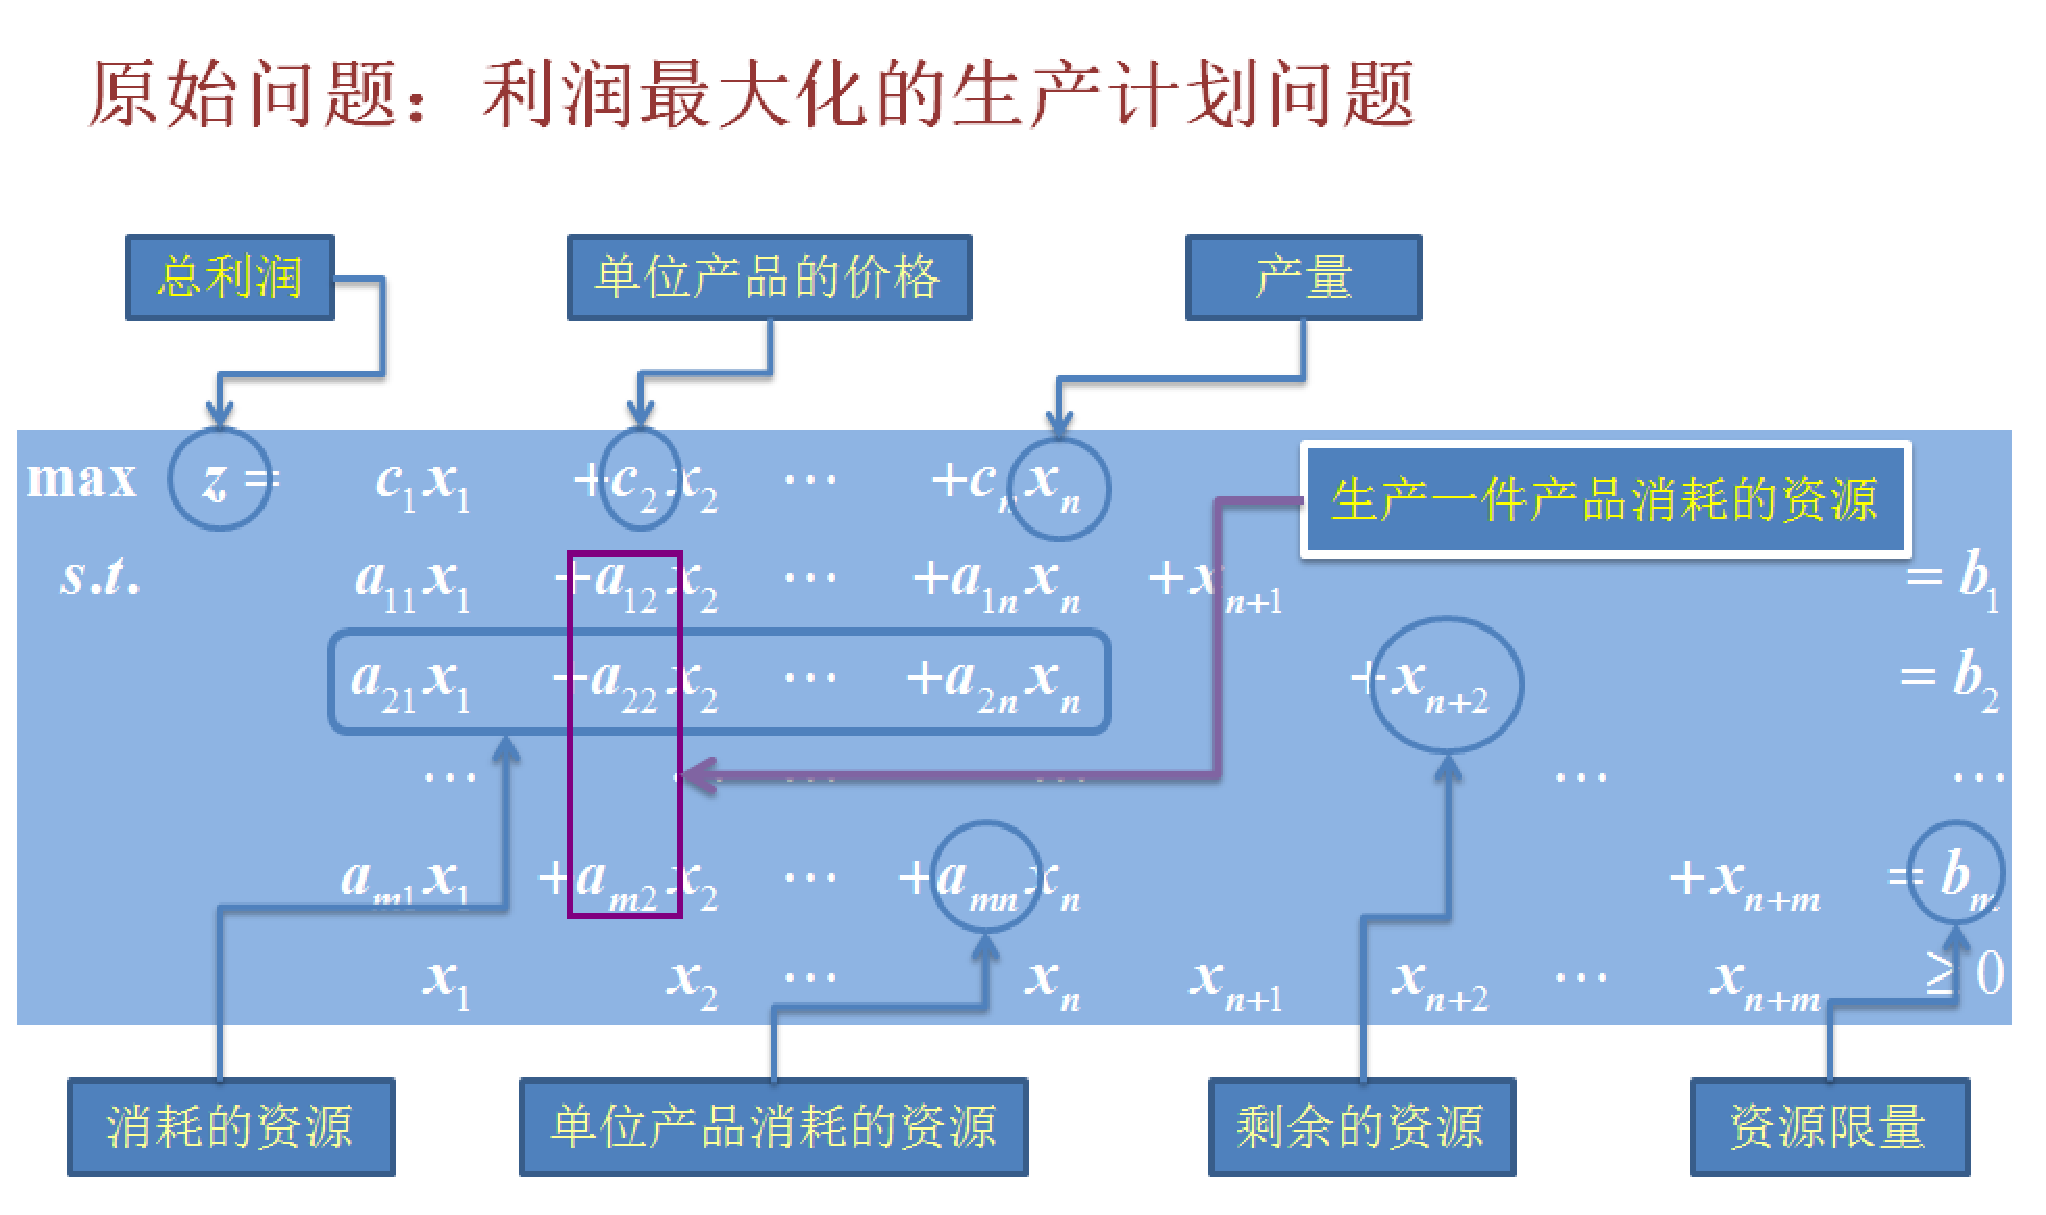
\includegraphics[width=0.9\textwidth]{figures/primal.eps}
\caption{原始问题:利润最大化的生产计划问题}\label{fig:primal}
\end{minipage}
\begin{minipage}[t]{0.49\linewidth}
\centering
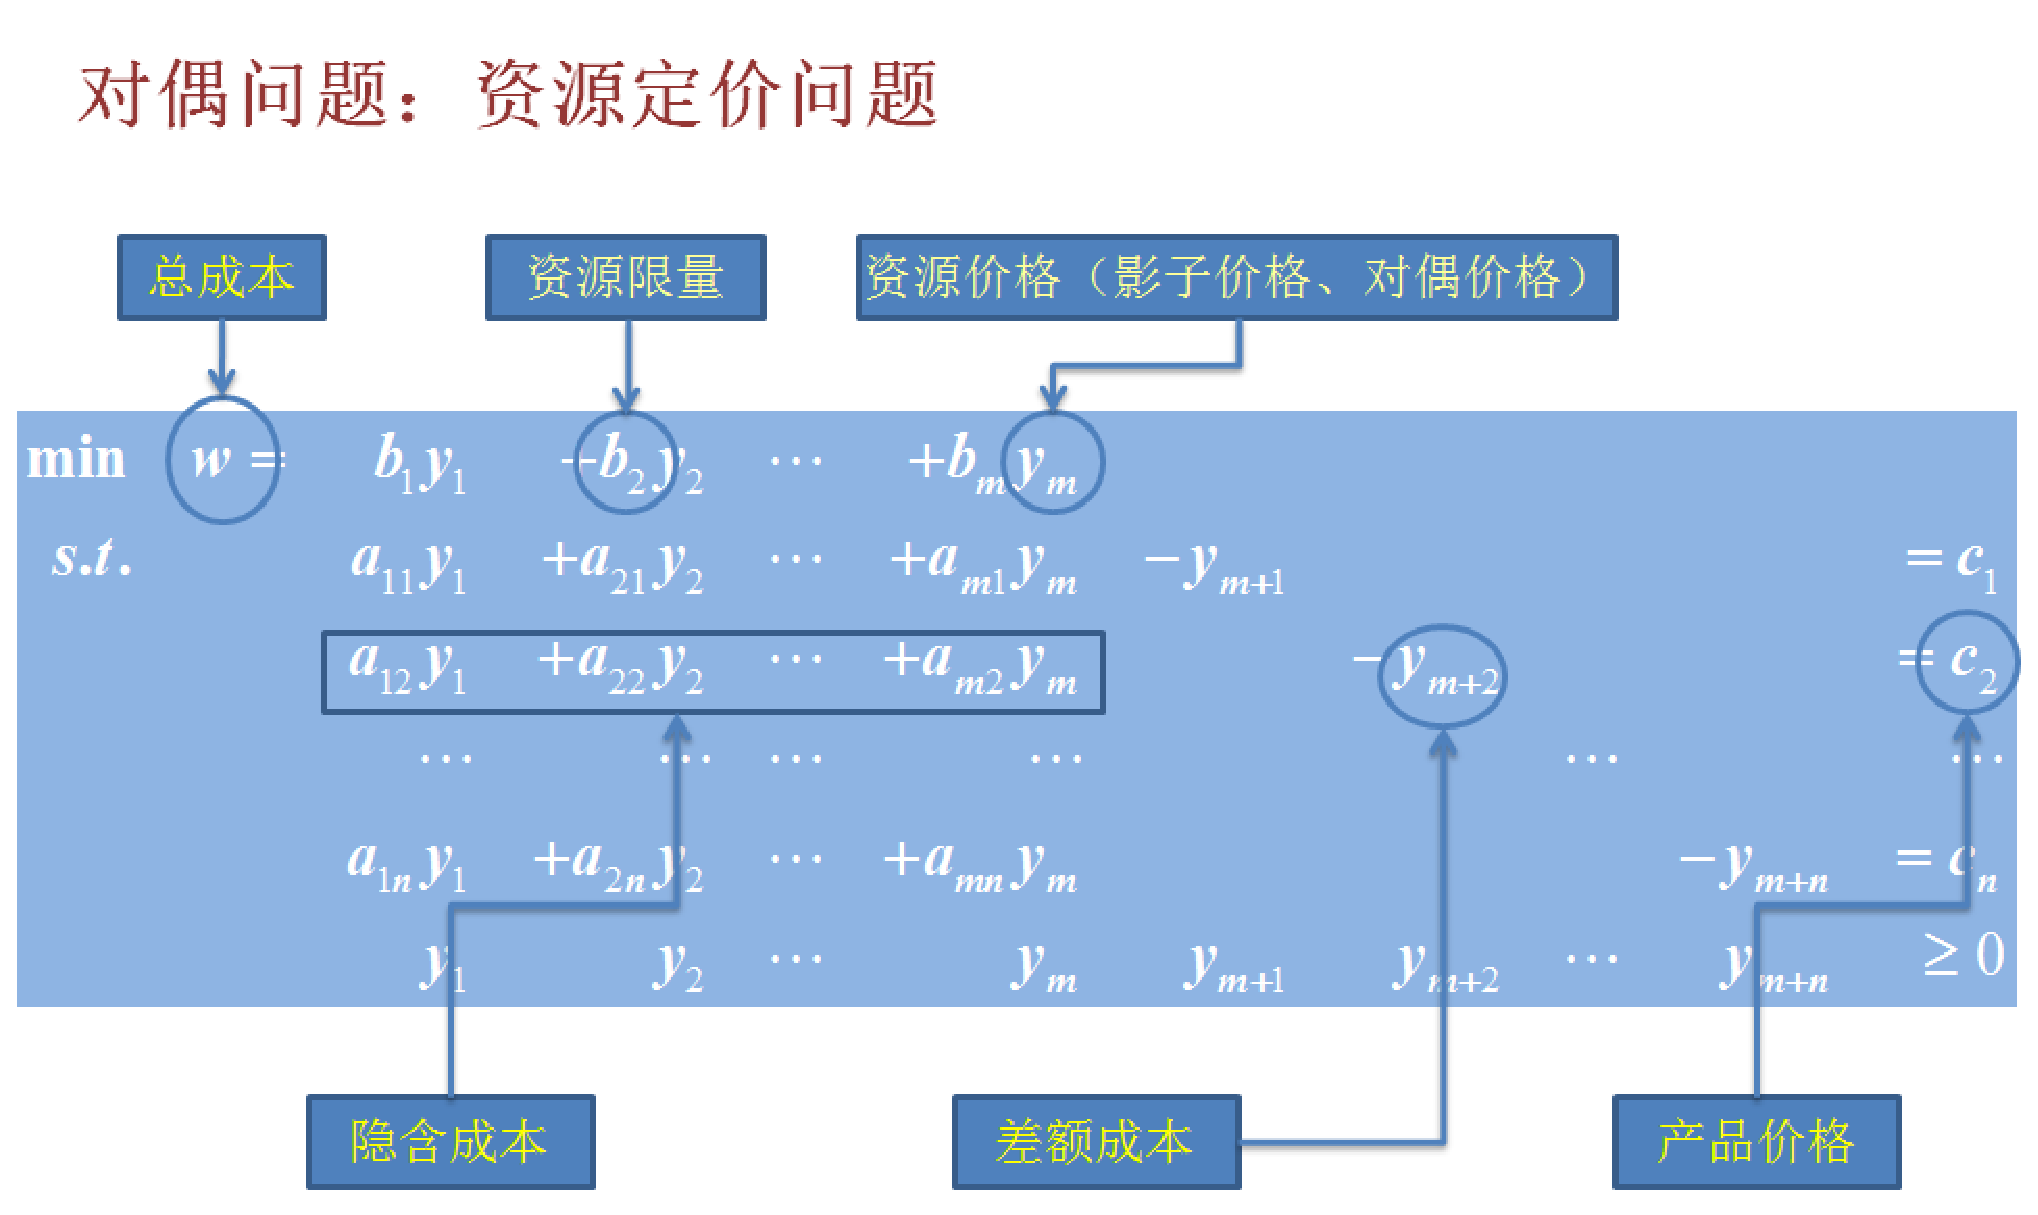
\includegraphics[width=0.9\textwidth]{figures/dual.eps}
\caption{对偶问题:成本最小化的资源定价问题}\label{fig:dual}
\end{minipage}
\end{figure}

在利润最大化的生产计划问题中(见图\ref{fig:primal}),生产一个单位的第2种产品消耗的资源为$a_{12},\ldots, a_{m2}$,各种资源的影子价格由对偶问题\ref{fig:dual} 所反映,即$y_1,y_2,\ldots, y_m$,则生产第2种产品的机会成本(或隐含成本)可以计算:
\begin{equation}\label{eq:oppcost}
  a_{12}y_1 + \ldots + a_{m2}y_m
\end{equation}
如图\ref{fig:dual}所示,根据市场定价,一个单位第2种产品的价格是$c_2$,则生产一个单位某产品的隐含成本1单位该产品的价格之间的差即是差额成本:
\begin{equation}\label{eq:diffcost}
  y_{m+2} = a_{12}y_1 + \ldots + a_{m2}y_m - c_2 = -\sigma_2
\end{equation}

只有当单位产品的市场价格大于隐含成本时,有利可图,(单纯形法中的)检验数($\sigma_2$)为正,始安排生产(进基);否则不安排。如果价格等隐含成本,检验数为0,表明通过生产本产品增加总利润的可能性已不存在(某变量出基后不再进基)。

\section{单纯形法}\label{sec:simplexmethod}
1947年,美国数学家George Dantzig\cite{dantzig1998linear}提出一种解线性规划的迭代算法 -- 单纯形法(Simplex Method),它被评为20世纪十大算法之一。
\footnote{20世纪十大算法包括:Metropolis Algorithm for Monte Carlo\cite{beichl2000metropolis}, Simplex Method for Linear Programming\cite{nash2000dantzig}, Krylov Subspace Iteration Methods\cite{van2000krylov}, The Decompositional Approach to Matrix Computations\cite{stewart2000decompositional}, The Fortran Optimizing Compiler\cite{padua2000fortran}, QR Algorithm for Computing Eigenvalues\cite{parlett2000qr}, Quicksort Algorithm for Sorting\cite{jaja2000perspective}, Fast Fourier Transform\cite{rockmore2000fft}, Integer Relation Detection\cite{bailey2000integer}, Fast Multipole Method\cite{board2000fast}.}

单纯形法在初始表上重复进行初等行变换(Elementary Row Operation,ERO)、高斯消元,由于线性规划方程数目小于变量个数时出现不定解,单纯形法从线性方程组中寻找单纯形,
\footnote{一个$d$维空间$\mathbb{R}^d$中的单纯形$\mathcal{S}$定义为由$d+1$个顶点$x_1,\ldots, x_d\in \mathbb{R}^d$所构成的凸包(Convex Hull)。单纯形就是一种简单的几何形状,通过将$d$ 维空间中的$d+1$个顶点相连形成。比如,一维单纯形是一个边,二维单纯形是一个三角形,三维单纯形就是一个四面体。}
从每一个单纯形中确定一组解,根据单纯形对应的解对目标函数的改变方向,选择下一个单纯形,逐步趋于最值点。

首先考虑如下包含$n$个变量,$m$个约束的标准形式的线性规划问题:
\begin{equation}
  \begin{array}{ll}
  \textit{max} & z = c^Tx\\
  \textit{s.t.} & Ax = b\\
  & x \ge 0
  \end{array}
\end{equation}
其中,$A\in \mathbb{R}^{m\times n}$,一般地,$m\le n$。对于约束条件中包含不等式的情况,可以通过添加松弛变量(Slacks)或剩余变量(Surplus)将其转化为等式形式。

为方便计算,向模型中添加$m$个“人工变量(Artificial Variables)”:
\[
x_{n+i} = b_i - \sum_{j=1}^n{a_{ij}x_j}
\]
则人工变量非负。我们将$x_1,\ldots,x_n$称作非基变量,它们构成的集合记做$\textbf{N}$,$x_{n+1},\ldots,x_{n+m}$称作基变量,它们构成的集合记做$\textbf{B}$。由人工变量的构造可知,非基变量可由基变量线性表出。

在此基础上,可以构建如下形式的规划问题:
\begin{equation}
  \begin{array}{ll}
  \textit{max} & z= \sum\limits_{i\in \textbf{N}}{c_ix_i} \\
  \textit{s.t.} & x_i = b_i - \sum_{j = 1}^n{a_{ij}x_j} ,i\in \textbf{B}\\
  & x \ge 0
  \end{array}
\end{equation}

使用单纯形法求解线性规划问题的基本步骤:
\begin{enumerate}[(1)]
  \item 确定初始基可行解;
  \item 做最优性检验,通过,即是最优解,否则,转入下一步;
  \item 转换可行解,得到相邻的基可行解,转入上一步。
\end{enumerate}

在单纯形法中,原问题的最优解满足:
\begin{enumerate}[(1)]
  \item 是基本解
  \item 可行($X_B = B^{-1}b\ge 0$)
  \item 检验数$C - C_BB^{-1}A\le 0, YA\le C$,即对偶解可行
\end{enumerate}

根据线性规划的基本性质可知,当线性规划方程的数目小于变量个数时,规划问题存在不定解。使用单纯形法解线性规划时,如果线性规划变量个数小于约束条件的个数,则将其转换为对偶问题再求解。

单纯形法易于程序实现,而且容易使用,但是它只适用于可以转化为标准型的规划问题,此外算法迭代次数将随着约束和变量数目的增加而迅速上升。一般地,单纯形法需要$2n-3n$步迭代,其中$n$表示原问题中变量的个数。Karmarkar方法通常仅仅需要迭代次数在$10-100$次即可求解模型,显然在求解大规模问题时更具优势。

\section{内点法}
\textbf{内点法}(Interior Point Method),又称\textbf{牛顿障碍法}(Newton Barrier Method),由John von Neumann提出,后经由Narendra Karmarkar发展成为解线性规划的一个重要方法。

\begin{example}
考虑如下线性规划问题:
\begin{equation}
  \begin{array}{ll}
  \textit{max} & x_1 + x_2 \\
  \textit{s.t.} & 2px_1 + x_2 \le p^2 + 1, p = \{0, 0.1, 0.2, \ldots, 0.9, 1\}\\
  \end{array}
\end{equation}
使用内点法求解它的过程可见图\ref{fig:karmarkar}:
\begin{figure}[htbp]
  \centering
  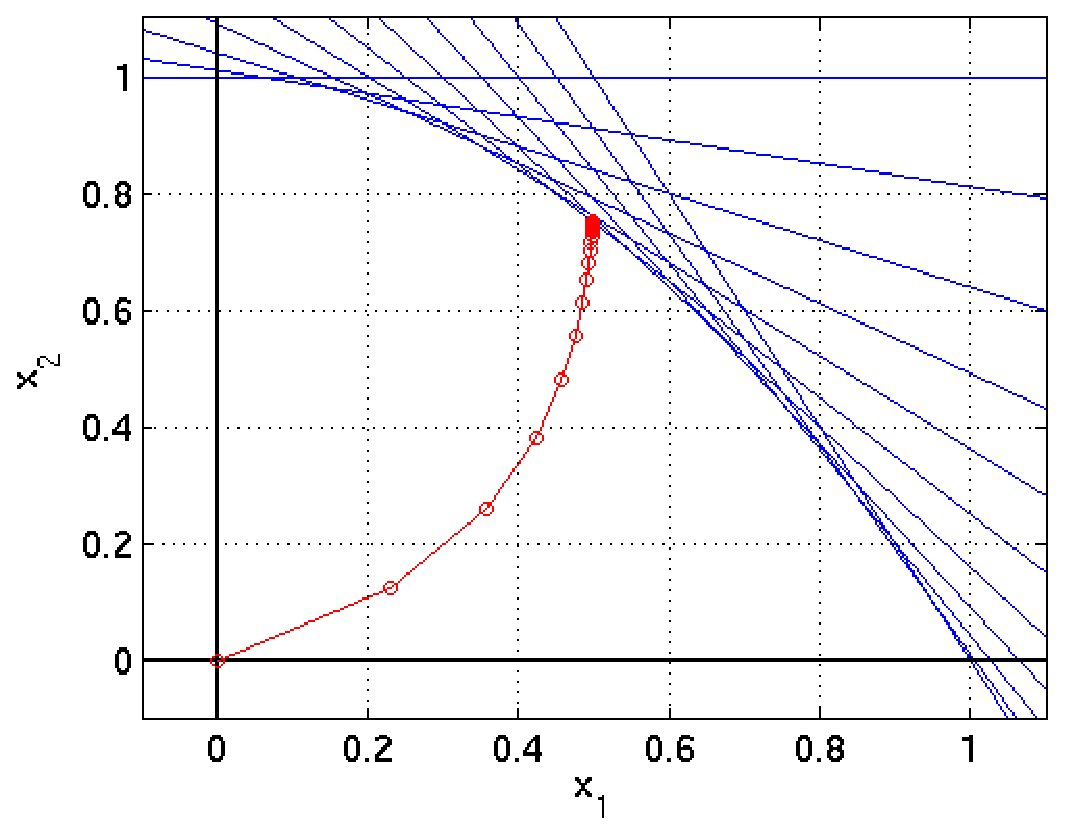
\includegraphics[width=0.6\textwidth, height=8cm]{figures/Karmarkar.eps}\\
  \caption{内点法求解示例}\label{fig:karmarkar}
\end{figure}
图中,蓝色的线表示约束条件,红色线是内点法求解路径。
\end{example}

\section{非线性规划}
在实际应用问题中,无论是问题规模还是变量个数都是庞大的,非线性程度越来越高,难以使用简单的线性模型予以刻画。通常,可以使用目标函数或约束条件至少有一个是非线性函数的数学规划表示,即非线性规划(Nonlinear Programming, NLP),一般可以表示成下面形式:
\begin{equation}\label{eq:nlpproblem}
    \begin{array}{lll}
      \textit{min} & f(x) \\
      \textit{s.t.} & g_i(x) \ge 0, i = 1, \ldots, m\\
       & h_j(x) = 0, j = 1,\ldots, l
    \end{array}
\end{equation}

一般认为,非线性规划诞生的重要标志是1951年Harold W. Kuhn与Albert W. Tucker发表的最优化条件(KT条件)
\cite{karush1939minima,kuhn1951nonlinear}。此后的50 年代主要是对梯度法和牛顿法的研究。在50 年代还发展了可分离规划和二次规划的多种解法,它们大都是以单纯形法为基础。50年代末到60年代末出现了许多解非线性规划问题的有效的算法,70年代又得到进一步的发展。非线性规划在工程、管理、经济、科研、军事等方面都有广泛的应用,为最优设计提供了有力的工具。20世纪80年代以来,计算机的飞速发展使非线性规划的研究如虎添翼,陆续诞生了信赖域法、稀疏拟牛顿法、内点法和有限存储法,在大规模非线性问题求解与并行计算方面也取得长足的发展。

非线性规划数值算法大致可分为\textbf{直接搜索算法}和\textbf{间接搜索算法}。直接搜索算法仅仅利用目标函数值信息直接建立搜索求解的方法,无须借助目标函数的梯度信息,因此又称作无梯度(Non-gradient)算法或零阶(Zeroth Order)算法。直接搜索算法包括随机搜索方法(Random Search)、网格搜索方法(Grid Search)、坐标轮换法(Univariate Search)\cite{desopo1959convex}、旋转坐标法(Rotating Coordinates)\cite{rosenbrock1960automatic}、模式方向法(Pattern Direction)\cite{hooke1961direct}、Powell方法\cite{powell1964efficient}和Nelder-Mead法\cite{nelder1965simplex}。
%遗传算法、差分进化和模拟退火算法
间接搜索算法需要利用一阶导数或黑塞矩阵(Hessian Matrix)信息,故又称为基于梯度的方法,典型的包括最速下降法、共轭梯度法(Fletcher-Reeves)、牛顿法、Marquardt方法、拟牛顿法、序列二次规划方法(Sequential Quadratic Programming, SQP)、增广拉格朗日方法(Augmented Lagrangian Method)和非线性内点法。非线性规划目前还没有适用于各种问题的一般算法,各个方法都有自己特定的适用范围。

%受Ford和Fulkson的关于多货物最大流网络规划问题的启发,1960年Dantzig与Wolfe发明了Dantzig-Wolfe分解原理,开创大规模系统最优化理论之先河,自问世以来在动态投入产出优化模型以为能源规划等许多领域得到广泛应用。

\subsection{基本概念}
由线性规划的性质我们知道,如果\textbf{线性规划}的最优解存在,其最优解只能在其可行域的边界上(特别是可行域的顶点上)达到。\textbf{非线性规划}的最优解(如果存在)则可能在其可行域的任意一点达到。

\begin{definition}[极小值点]
给定集合\textit{S}上的点$\hat x$,如果存在$\varepsilon \ge 0$,对于任意的$x\in $\textit{S},当$\|x-\hat x\| \le \varepsilon$时,都有$f(x) \ge f(\hat x)$,则称$\hat x$是函数$f$在\textit{S}上的\textbf{局部极小值点}。如果对任意的$x \in$ \textit{S},都有$f(x) \ge f(\hat x)$,则$\hat x$是函数$f$在
\textit{S}上的\textbf{全局极小值点}。
\end{definition}

\begin{definition}[驻点、临界点、拐点、鞍点]
如果函数$f$在某点$\hat x$处不可微或$f'(\hat x) = 0$,则称$\hat x$是\textbf{临界点}(Critical Point),对应函数值称作是临界值。如果函数是一阶可导的,且$f'(\hat x) = 0$,则称点$\hat x$ 是\textbf{驻点}(Stationary Point)。如果函数在$\hat x$处由凹变凸或由凸变凹,则称$\hat x$是函数的一个\textbf{拐点}
(Inflection Point),同时如果$f(\hat x)=0$,则称$\hat x$ 是\textbf{鞍点}(Saddle Point)。
\end{definition}

\begin{theorem}[费马定理]
给定函数$f:(a,b) \mapsto \mathbb R$,如果$\hat x\in(a,b)$是$f$的一个局部极值点,若$f$在$\hat x$处是可微的,则$f'(\hat x) = 0$。
\end{theorem}

\begin{definition}[有效约束和无效约束]
假设$x$是非线性规划的一个可行解,它自然满足所有的约束。考虑某不等式约束条件$g_i(x)\ge 0$。当$g_i(x)=0$时,点$x$处于此约束条件形成的可行域边界上,约束条件对点$x$的微小摄动构成限制,则称此约束条件是点$x$的\textbf{有效约束}(active);反之,当$g_i(x)>0$时,约束条件对点$x$的微小摄动(small variation)不会构成限制,则称此约束条件是点$x$的\textbf{无效约束}(inactive)。所有的等式约束条件都是点$x$的有效约束。
\end{definition}

\begin{definition}[可行方向]
假设$x_0$是非线性规划的一个可行解,若存在$\delta>0$,对任意的$\lambda\in (0,\delta)$,$x_0+\lambda d$仍处于可行域上,则称$d$是$x_0$的一个\textbf{可行方向}。
\end{definition}

将$g_i(x)$在点$x_0$处作一阶泰勒展开,由
\[
    g_i(x_0+\lambda d) = g_i(x_0) + \lambda d^T \nabla g_i(x_0) + O(\lambda)
\]
可知满足\textcolor{red}{$d^T \nabla g_i(x_0) \ge 0,i=1,\ldots,m$ 的方向$d$是点$x_0$的一个可行方向}。

\begin{definition}[下降方向]
假设$x_0$是非线性规划的一个可行解,若存在$\delta>0$,对任意的$\lambda\in (0,\delta)$都有$f(x_0+\lambda d)<f(x_0)$,则称$d$是$x_0$的一个\textbf{下降方向}。
\end{definition}

将$f(x)$在点$x_0$处作一阶泰勒展开,由
\[
    f(x_0+\lambda d) = f(x_0) + \lambda d^T \nabla f(x_0) + O(\lambda)
\]
可知满足$d^T \nabla f(x_0) < 0$的方向$d$是点$x_0$的一个下降方向。

\begin{definition}[正则点]
给定某可行解$x$,如果所有有效的不等式约束函数与等式约束函数在$x$处的梯度线性无关,则称点$x$是\textbf{正则点}(Regular Point)。
\end{definition}

根据定义可知,从某点出发,沿任意可行方向(距离很小)都不能使目标函数值减少,则该点即局部极小值点。

\begin{theorem}[最优化的必要性条件]
假设$\hat x$是目标函数$f:\mathbb R^n \mapsto \mathbb{R}$的无约束最小值点,$f$是含$\hat x$的开集\textit{S}上的一阶连续可微函数,则满足\textbf{一阶必要性条件},即$\nabla f(\hat x) = 0$。如果$f$又是二阶连续可微的,则满足\textbf{二阶必要性条件},即$\nabla^2 f(\hat x)$半正定。
\end{theorem}

\section{拉格朗日乘子法}
拉格朗日乘子法(Lagrange Multiplier Method)主要用于解决等式约束的优化问题
\begin{equation}
    \begin{array}{lll}
      \textit{min} & f(x) \\
      \textit{s.t.} & h_i(x) = 0,~~i = 1,\ldots,m
    \end{array}
\end{equation}
其中,$x\in\mathbb{R}^n$,目标函数$f:\mathbb{R}^n \mapsto \mathbb{R}$是一阶连续可微函数。

我们知道,可行域上目标函数$f$的极小值点应当是一个驻点\footnote{Stationary Point:函数在该点处的梯度为零},对于可行域上驻点存在一个有用的性质:
\begin{theorem}
点$x$是可行域上驻点的充要条件是:沿任意可行方向移动点$x$,目标函数值都不会发生改变。
\end{theorem}

给定点$x$,设$V$是保持目标函数值不变的方向集,则从$x$出发不改变目标函数值的任意移动方向皆垂直于目标函数在该点处的梯度。对任意的$v\in V\subset \mathbb{R}^n$,都有等式
\begin{equation}
    v^T \nabla f(x) = 0
\end{equation}
成立。

规划问题中的约束条件限制了点$x$可以移动的方向:同时满足所有的等式约束,不会改变函数$g_i$的值。设$V'$是$x$的可行方向集合,那么从$x$出发不“违背”约束条件的任何移动方向都垂直于约束函数的梯度。对任意的$v\in V'\subset \mathbb{R}^n$,都有等式
\begin{equation}
    v^T \nabla h_i(x) = 0, i = 1,\ldots,m
\end{equation}
成立。我们由此得出结论:
\begin{theorem}
点$x$是可行域上驻点的充要条件是:沿任意方向移动点$x$,如果它改变了目标函数的值,则它至少会违背一个约束条件。
\end{theorem}

假设存在某个从$x$ 出发的移动方向,如果它是可行方向,即满足所有的约束条件,而且在移动后,目标函数值发生改变,无论是变大还是变小,皆表明$x$ 并非可行域上的驻点,矛盾产生。换句话说,目标函数在可行域上驻点$x$处的梯度垂直于由$V'$生成的子集,而后者又与约束函数在$x$处的梯度垂直。

\begin{theorem}[拉格朗日乘子定理]
假设$x^*$是目标函数$f$的局部极小值点,若约束函数的梯度向量组$h_1(x^*),\ldots, h_m(x^*)$\textbf{线性无关}($x^*$是一个正则点),则存在唯一的拉格朗日乘子向量$\Lambda^* = (\lambda_1^*,\ldots,\lambda_m^*)$使得等式
\begin{equation}
    \nabla f(x^*) + \sum\limits_{i=1}^m \lambda_i^* \nabla h_i(x^*) =0
\end{equation}
成立。

如果$f$与$h_i,i=1,\ldots,m$都是二阶连续可微的,则对任意$v\in V(x^*)$
\begin{equation}
    v^T (\nabla^2 f(x^*) + \sum\limits_{i=1}^m \lambda_i^* \nabla^2 h_i(x^*)) v \ge 0
\end{equation}
其中,$V(x^*) = \big\{v\mid v^T \nabla h_i(x^*)=0, i = 1,\ldots,m\big\}$。
\end{theorem}

\begin{proof}
我们下面利用罚函数法(Penalty Approach)给出证明~\cite{bertsekas1999nonlinear}。对于含有等式约束的非线性规划问题,我们通过对违反约束条件的点施加惩罚,将有约束最优化问题转化为无约束最优化问题。为了方便表示,令$h=(h_1,h_2,\ldots,h_m)^T$。

对于$k=1,2,\ldots$,定义函数:
\begin{equation}
    F_k(x) = f(x) + \frac{k}{2} \|h(x)\|^2 + \frac{\alpha}{2} \|x-x^*\|^2
\end{equation}
其中,$x^*$表示约束问题的局部极小值点,$\alpha>0$。第二项是对违反约束条件的点$h(x)=0$施加的惩罚项,第三项则确保$x^*$是
\[
    \begin{array}{ll}
      \textit{min} & f(x) +  \frac{\alpha}{2} \|x-x^*\|^2 \\
      \textit{s.t.} & h(x) = 0
    \end{array}
\]
严格局部极小值点。

由于$x^*$是一个局部极小值点,我们可以选择半径$\varepsilon>0$,使得封闭球
\begin{equation}
    S = \{x\mid \|x-x^*\| \le \varepsilon\}
\end{equation}
内所有可行解$x$,都有$f(x^*) \le f(x)$。

对于约束优化问题
\begin{equation}\label{eq:constainedlagrange}
    \begin{array}{ll}
      \textit{min} & F_k(x) \\
      \textit{s.t.} & x\in S
    \end{array}
\end{equation}
假设其最优解是$x^k$,对于所有的$k$,则有
\begin{equation}\label{neq:bound}
    F_k(x^k) = f(x^k) +  \frac{k}{2} \|h(x^k)\|^2 + \frac{\alpha}{2} \|x^k-x^*\|^2 \le F_k(x^*) = f(x^*)
\end{equation}
由$f(x^k)$在$S$上有界,可知$\lim\limits_{k\rightarrow \infty} h(x^k) = 0$(否则,左端无界,矛盾)。对于每个极限值$\bar{x} = \lim\limits_{k\rightarrow \infty} x^k$,都有$h(\bar{x}) = 0$,从而对不等式~\ref{neq:bound} 两边同时取极限可得:
\begin{equation}
    f(\bar{x}) + \frac{\alpha}{2} \|\bar{x}-x^*\|^2 \le f(x^*)
\end{equation}
由于$\bar{x}\in S$上的可行解,所以$f(x^*) \le f(\bar{x})$,那么$\bar{x} = x^*$,表明当$k$充分大时,$x^k$是$F_k(x)$的无约束局部极小值点。

下面我们利用无约束优化的相关性质证明拉格朗日乘子定理:根据一阶必要条件,当$k$充分大时,有
\begin{equation}\label{eq:lagrangenecessary}
    0 = \nabla F_k(x^k) = \nabla f(x^k) + k \nabla h(x^k) h(x^k) + \alpha (x^k - x^*)
\end{equation}
成立。

由于$\nabla h(x^*)$的秩为$m$,当$k$充分大时$\nabla h(x^k)$有相同的结论,所以$\nabla h(x^k)^T \nabla h(x^k)$ 可逆,那么对于上式,整理可得:
\begin{equation}
    kh(x^k) = -(\nabla h(x^k)^T \nabla h(x^k))^{-1} \nabla h(x^k)^T \big[\nabla f(x^k) + \alpha (x^k - x^*)\big]
\end{equation}
两边同时取极限可知
\begin{equation}
    \lim\limits_{k\rightarrow \infty} kh(x^k) = \Lambda^* = -(\nabla h(x^*)^T \nabla h(x^*))^{-1} \nabla h(x^*)^T \nabla f(x^*)
\end{equation}
根据等式~\eqref{eq:lagrangenecessary}可得
\begin{equation}
    \nabla f(x^*) + \Lambda^* \nabla h(x^*) = 0
\end{equation}
由此证明了一阶优化条件。

对于$F_k(x)$,根据其二阶优化条件可知,当$k$充分大时,对任意的$\alpha>0$,矩阵
\begin{equation}
    \nabla^2 F_k(x^k) = \nabla^2 f(x^k) + k \nabla h(x^k) (\nabla h(x^k))^T + k \sum\limits_{i=1}^m h_i(x^k) \nabla^2 h_i(x^k) + \alpha I
\end{equation}
是半正定的。给定$v\in V(x^*)$,则$v^T \nabla h(x^*) = 0$,取$v^k$表示$v$在$(\nabla h(x^k))^T$零子空间上的投影,则
\begin{equation}
    v^k = v - \nabla h(x^k)\big[(\nabla h(x^k))^T \nabla h(x^k)\big]^{-1} v^T \nabla h(x^k)
\end{equation}
已知$(v^k)^T \nabla h(x^k)=0$,$\nabla^2 F_k(x^k)$半正定,可得
\begin{equation}
    0\le (v^k)^T \nabla^2 F_k(x^k) v^k = (v^k)^T \big[\nabla^2 f(x^k) + k \sum\limits_{i=1}^m h_i(x^k) \nabla^2 h_i(x^k) \big] v^k + \alpha \|v^k\|^2
\end{equation}
由于$x^k\rightarrow x^*$,$kh_i(x^k)\rightarrow \lambda_i^*$,并且$v^T \nabla h(x^*)=0$,则$v^k\rightarrow v$,对任意的$v\in V(x^*)$,都有
\begin{equation}
    0\le v^T \big[\nabla^2 f(x^*) + \sum\limits_{i=1}^m \lambda_i^* \nabla^2 h_i(x^*) \big] v + \alpha \|v\|^2
\end{equation}

参数$\alpha$可以取任意小的正数,则对任意的$v\in V(x^*)$有
\begin{equation}
    0\le v^T \big[\nabla^2 f(x^*) + \sum\limits_{i=1}^m \lambda_i^* \nabla^2 h_i(x^*) \big] v
\end{equation}
证毕。
\end{proof}

根据一阶必要条件和等式约束条件,由$m+n$个方程构建的包含$m+n$ 个未知数的方程组,并确定出唯一解。对于一阶必要条件,要求约束函数的梯度向量组线性无关,如果是线性相关的,那么会产生什么影响呢?我们下面给出一个例子说明这个问题:
\begin{equation}
    \begin{array}{lll}
      \textit{min} & f(x) = x_1 +  x_2 \\
      \textit{s.t.} & h_1(x) = (x_1-1)^2 + x_2^2 - 1 = 0 \\
       & h_2(x) = (x_1-1)^2 + x_2^2 - 4 = 0
    \end{array}
\end{equation}
它只包含一个可行点$(0,0)$,并且是极小值点,两个约束函数的梯度是线性相关的,因此对于任意的$\lambda_1,\lambda_2$,等式
\[
    \nabla f(x^*) + \lambda_1 \nabla h_1(x^*) + \lambda_2 \nabla h_2(x^*) = 0
\]
始终不成立。

\begin{theorem}[充分条件]
假设$f$和$g$是二阶连续可微函数,定义拉格朗日函数
\begin{equation}
    L(x,\Lambda) = f(x) + \Lambda^T h(x)
\end{equation}
设$x^*\in \mathbb{R}^n$,$\Lambda^*\in \mathbb{R}^m$满足
\begin{equation}
    \begin{array}{lll}
      \nabla_x L(x^*,\Lambda^*) & = & 0 \\
      \nabla_{\Lambda} L(x^*,\Lambda^*) & = & 0
    \end{array}
\end{equation}
并且对任意的$v\ne 0$,当$v^T \nabla h(x^*) = 0$时,
\begin{equation}
    v^T \nabla_{xx}^2 L(x^*,\Lambda^*) v > 0
\end{equation}
则$x^*$是非线性等式约束优化问题的严格局部最小值点。
\end{theorem}

充分条件可以使用罚函数法或者可行方向法予以证明~\cite{bertsekas1999nonlinear}。
\subsection{对偶问题与KKT条件}
KKT(Karush-Kuhn-Tucker)条件,又称KT(Kuhn-Tucker)条件,是非线性规划的一个重要结论。早在1939 年,William Karush\cite{karush1939minima} 在其博士论文中就得到这一结论,然而直到Harold W. Kuhn与Albert W. Tucker在1951 年首次公开发表\cite{kuhn1951nonlinear},人们才意识到这一工作的重要性。

KKT条件是对拉格朗日乘子法(Lagrange Multipliers Method)的推广,对于包含不等式约束条件的非线性规划问题:
\begin{equation}\label{eq:nlp}
    \begin{array}{lll}
      \textit{min} & f(x) \\
      \textit{s.t.} & g_i(x) \le 0, i = 1, \ldots, m\\
       & h_j(x) = 0, j = 1,\ldots, l
    \end{array}
\end{equation}
其中,$x\in \mathbb{R}^n$,$f:\mathbb{R}^n \mapsto \mathbb{R}$是目标函数,$g_i:\mathbb{R}^n \mapsto \mathbb{R},(i=1,\ldots,m)$是不等式约束函数,$h_j:\mathbb{R}^n \mapsto \mathbb{R},(j=1,\ldots,l)$是等式约束函数,都是一阶连续可微函数。

构造拉格朗日函数
\begin{equation}
    L(x,\alpha,\beta) = f(x) + \sum\limits_{i=1}^m \alpha_i g_i(x) + \sum\limits_{j=1}^l \beta_j h_j(x)
\end{equation}
其中,$\alpha\ge 0,\beta$为拉格朗日乘子向量。

记$\Theta_p(x) = \max\limits_{\alpha \ge 0,\beta} L(x,\alpha,\beta)$,由于
\begin{equation}
   \max\limits_{\alpha \ge 0,\beta} L(x,\alpha,\beta) =  f(x) + \max\limits_{\alpha \ge 0,\beta} \bigg[\sum\limits_{i=1}^m \alpha_i g_i(x) + \sum\limits_{j=1}^l \beta_j h_j(x) \bigg]
\end{equation}
\begin{itemize}
  \item 当$x$是可行解时,满足所有约束条件,则$h_j(x)=0,j=1,\ldots,l$,函数$\Theta_p(x)$可简化为
  \[
    \Theta_p(x) = f(x) + \max\limits_{\alpha \ge 0,\beta} \sum\limits_{i=1}^m \alpha_i g_i(x)
  \]
  由于$g_i(x)\le 0,i=1,\ldots,m,\alpha \ge 0$,则$\sum\limits_{i=1}^m \alpha_i g_i(x) \le 0$,当且仅当$\alpha=0$时等式成立,从而$\Theta_p(x) = f(x)$。
  \item 当$x$不可行时,违反至少一个约束条件,则通过灵活选择$\alpha,\beta$可得$\Theta_p(x)=\infty$。
\end{itemize}
综上可得
\begin{equation}
    \Theta_p(x) = \max\limits_{\alpha \ge 0,\beta} L(x,\alpha,\beta) = \left\{
        \begin{array}{lll}
          f(x) & x\text{是可行解} \\
          \infty & \text{否则}
        \end{array}
    \right.
\end{equation}
利用拉格朗日函数可以建立如下无约束最优化问题
\begin{equation}\label{eq:lagrangeprimal}
    \hat p = \min\limits_x \Theta_p(x) = \min\limits_x \max\limits_{\alpha\ge 0,\beta} L(x,\alpha,\beta)
\end{equation}
它与原始问题\eqref{eq:nlp}等价(解相同),我们称其为原问题。
如果记$\Theta_d(\alpha,\beta) = \min\limits_x L(x,\alpha,\beta)$,容易证明$\Theta_d(\alpha,\beta) \le \hat p$。假设$x_0$是问题\eqref{eq:lagrangeprimal} 的任意可行解,即$g_i(x_0)\le 0, h_j(x_0)=0, \alpha \ge 0$,则有
\begin{equation}
    \sum\limits_{i=1}^m \alpha_i g_i(x_0) + \sum\limits_{j=1}^l \beta h_j(x_0) \le 0
\end{equation}
从而
\begin{equation}
    L(x_0,\alpha,\beta) = f(x_0) + \sum\limits_{i=1}^m \alpha_i g_i(x_0) + \sum\limits_{j=1}^l \beta h_j(x_0) \le f(x_0)
\end{equation}
也就是说
\begin{equation}
    \Theta_d(\alpha,\beta)= \min\limits_x L(x,\alpha,\beta) \le L(x_0,\alpha,\beta) \le f(x_0)
\end{equation}
由$x_0$的任意性可知,$\Theta_d(\alpha,\beta) \le \hat p$成立。

对于下面形式的问题
\begin{equation}\label{eq:lagrangedual}
    \hat d = \max\limits_{\alpha\ge 0,\beta} \Theta_d(\alpha,\beta) = \max\limits_{\alpha\ge 0,\beta} \min\limits_x L(x,\alpha,\beta)
\end{equation}
构成原问题的对偶问题,必然有
\begin{equation}\label{eq:weakduality}
    \hat d\le \hat p \text{(\textbf{弱对偶性},Weak Duality)}
\end{equation}
差值$\hat p - \hat d$称为\textbf{对偶间隙(Duality Gap)},当对偶间隙为零时
\begin{equation}\label{eq:strongduality}
    \hat d =\hat p \text{(\textbf{强对偶性},Strong Duality)}
\end{equation}

当强对偶性成立时,原问题的最优解是$\hat x$,对偶问题的最优解是$\hat \alpha,\hat\beta$,则拉格朗日函数在可行解$(\hat x,\hat\alpha,\hat\beta)$的函数值同原始问题目标函数值$f(\hat x)$相等,即
\begin{equation}
    L(\hat x,\hat\alpha,\hat\beta) = f(\hat x) + \sum\limits_{i=1}^m \hat\alpha_i g_i(\hat x) + \sum\limits_{j=1}^l \hat\beta_j h_j(\hat x) = f(\hat x)
\end{equation}
\begin{itemize}
  \item $\hat x$是$\Theta_p(x)$的极值点,由拉格朗日函数与$\Theta_p(x)$的定义,极值点的必要条件,可得
    \begin{equation}
        \nabla f(\hat x) + \sum\limits_{i=1}^m \hat\alpha_i \nabla g_i(\hat x) + \sum\limits_{j=1}^l \hat\beta_j \nabla h_j(\hat x) = 0
    \end{equation}
  我们称之为\textbf{平稳性(Stationarity)条件}。
  \item $\hat x$是原始问题的可行解,满足$h_j(\hat x)=0,j=1,\ldots,l$,所以
    \begin{equation}
        \sum\limits_{i=1}^m \hat\alpha_i g_i(\hat x) = 0
    \end{equation}
  既然$\hat\alpha_i g_i(\hat x)\le 0,\forall i$,则有
    \begin{equation}
        \hat\alpha_i g_i(\hat x) = 0, i = 1,\ldots, m
    \end{equation}
  我们称之为\textbf{互补松弛(Complementary Slackness)条件},当$\hat\alpha_i>0$时,必然有$g_i(\hat x)=0$,表明此不等式约束条件是有效的。
\end{itemize}

\subsubsection{必要条件}
如果$\hat x$是极小值点,并且满足一些约束规范条件(Constraint Qualification,Regularity Conditions),则存在拉格朗日乘子向量$\hat \alpha \in \mathbb{R}^m,\beta\in \mathbb{R}^l$,满足下面几条性质(统称为KKT优化条件):
\begin{itemize}
  \item \textbf{主可行性条件}(Primal Feasibility Conditions)
  \begin{equation}
    \begin{array}{ccc}
      g_i(\hat x) & \le & 0 \\
      h_j(\hat x) & = & 0
    \end{array}
  \end{equation}
  \item \textbf{对偶可行性条件}(Dual Feasibility Condition)
  \begin{equation}
    \hat\alpha_i \ge 0
  \end{equation}
  \item \textbf{互补松弛条件}
  \begin{equation}
    \hat\alpha_i g_i(\hat x) = 0
  \end{equation}
  \item \textbf{平稳性条件}
  \begin{equation}
    \nabla f(\hat x) + \sum\limits_{i=1}^m \hat\alpha_i \nabla g_i(\hat x) + \sum\limits_{j=1}^l \hat\beta_j \nabla h_j(\hat x)=0
  \end{equation}
\end{itemize}
其中,$i = 1, \ldots, m, j = 1,\ldots, l$。特别地,当$m=0$时,非线性规划仅含等式约束,则KTT条件退化为拉格朗日条件。

\subsubsection{约束规范条件}
对于极值点$\hat x$,若满足KKT必要性条件,必需满足一些约束规范条件。常用的约束规范条件有
\begin{itemize}
  \item 线性无关约束规范条件(Linear Independence Constraint Qualification, LICQ):有效不等式约束函数与等式约束函数在$\hat x$处的梯度线性无关(正则点)
  \item Slater约束规范条件:对于凸优化问题,所有的有效不等式约束在点$\hat x$处是严格不等式
\end{itemize}

\subsubsection{充分条件}
假设目标函数$f$与不等式约束函数$g_i(i=1,\ldots,m)$都是凸函数,等式约束函数$h_j(j=1,\ldots,l)$是仿射函数,$\hat x$是一个可行解,如果存在$0\le \hat\alpha \in \mathbb{R}^m,\beta\in \mathbb{R}^l$,满足\textbf{互补松弛}与\textbf{平稳性}条件,则$\hat x$是\textbf{全局极小值点}。

\subsubsection{Fritz John必要条件}
对于非线性优化问题
\begin{equation}
    \begin{array}{lll}
      \textit{min} & f(x) \\
      \textit{s.t.} & g_i(x) \le 0, i = 1, \ldots, m\\
    \end{array}
\end{equation}
根据Farkas引理,设$\hat x$是一个局部极小值点,则存在不全为零的拉格朗日乘子$\hat \lambda_i,i=0,1,\ldots,m$,满足下面几个性质(统称Fritz John必要条件)
\begin{equation}\label{eq:fritzjohn}
    \begin{array}{rcl}
      \hat \lambda_0 \nabla f(\hat x) + \sum\limits_{i=1}^m \hat\lambda_i \nabla g_i(\hat x) &=& 0 \\
      \hat \lambda_i &\ge& 0,~~i = 0,1,\ldots,m \\
      \hat \lambda_i g_i(\hat x) &=& 0,~~i = 1,2,\ldots,m
    \end{array}
\end{equation}

当原问题比较复杂,而对偶问题具有良好的结构时,利用原问题的强对偶性“通过求解对偶问题实现对原问题的求解”是一种常用的优化方法,比如当目标函数与不等式约束函数都是凸函数,等式约束函数是仿射函数,而不等式约束条件是严格的,则相应的优化问题是强对偶的。一般而言,KKT条件是强对偶性成立的必要条件,特别地,当原问题是凸优化问题时,KKT条件是强对偶性成立的充分必要条件。

\section{梯度下降法}
\textbf{梯度下降法}(Gradient Descent Method),又称\textbf{最速下降法}(Steepest Descent Method),由大数学家Cauchy于1847年最先使用。它是最古老的一种解析方法,而其他解析方法大多承其衣钵,并构成最优化方法的基础。梯度下降法的优点是工作量少,存储变量少,对初始点不敏感。当然,它也有缺点。比如,对于多峰形式(Multi-Modal)的参数分布,它的收敛速度很慢,容易陷入局部最优点。

如果我们希望利用迭代算法寻找二阶可微函数$f$的最小点,假设当前最优点是$x_k\in \mathbb{R}^n$,在选择下一个点 $x_{k+1} = x_k + \alpha h$ 时,遵循的原则或目标是能够最小化函数值
$f(x_{k+1})$,即
\begin{equation}\label{eq:gradientdescent}
    \begin{array}{ll}
        \min\limits_{h \in \mathbb{R}^n} & f(x_{k+1}) = f(x_k + \alpha h)
    \end{array}
\end{equation}
其中,$h$表示搜索的方向,一般地$\|h\| = 1$,$\alpha>0$表示步长或者学习率(Learning Rate)。

根据泰勒展开公式有:
\[
    f(x_k + \alpha h) = f(x_k) + \alpha g(x_k)^T h + O(\alpha)
\]
其中,$g(x_k) = \nabla f(x_k)$。

不考虑高阶部分,等式\eqref{eq:gradientdescent}等价于最小化$g(x_k)^T h$。根据内积公式可知,当$h = -g(x_k) = -\nabla f(x_k)$ (负梯度方向)时,$f(x_k)$下降的速度最快(最速下降法由此而来)。

梯度下降法在机器学习中有广泛的应用,比如在监督型学习算法中,根据经验风险最小化原则训练模型就可能用到梯度下降法。假设预测模型一阶可微$f=f(\omega,x)$,则预测模型在数据集$S=\{x_i,y_i\}_{i=1}^n$上的经验损失
\begin{equation}
    L(\omega,S) = \frac{1}{n} \sum\limits_{i=1}^n \ell(y_i,f(\omega,x_i))
\end{equation}
其中,$\ell(y,f(\omega,x))$是预测模型在单个样本上的损失函数,假设它是一阶可微的。

根据梯度下降法有下面的参数更新法则有:
\begin{equation}
    \omega_{t+1} = \omega_t + \alpha \frac{1}{n} \sum\limits_{i=1}^n \nabla L(y_i, f(\omega,x_i))
\end{equation}
由于每次更新模型参数时,都要用到所有的训练样本,梯度下降法也称\textbf{批量梯度下降法}。批量梯度下降法在更新参数时,用到了数据集中全部的样本,时间复杂度为$O(n)$。

在大数据处理时,对于某些类型的损失函数,计算所有样本的平均梯度值是不可行的。为此,研究人员提议使用随机抽取的单个样本计算近似的平均梯度值,利用它来更新模型参数,能够在大幅减少单次迭代计算量的同时,还能取得同批量梯度下降法相似的效果,这种方法被称作\textbf{随机梯度下降法},也称\textbf{增量随机梯度下降法}。

假设随机选取的样本是$x_0$,则使用下面的公式更新参数:
\begin{equation}
    \omega_{t+1} = \omega_t + \alpha_t \nabla L(y_0, f(\omega,x_0))
\end{equation}
为保证收敛,通常要求学习率$\alpha_t$序列满足
\begin{equation}
    \sum\limits_{t=1}^T \alpha_t = \infty,~~\sum\limits_{t=1}^T \alpha_t^2 < \infty
\end{equation}
一般选择$\alpha_t=1/t$或$\alpha_t=\alpha_0(1+\lambda\alpha_0)^{-1}$。

随机梯度下降法由于单次迭代计算量小,效率很高,远优于经典的优化算法,如牛顿法,特别适合大数据机器学习\cite{bottou2010large}。它也存在一些缺陷,比如在迭代过程中产生许多噪声、每次迭代的搜索方向未必是整体梯度下降的方向等。随机梯度下降法已经被用于训练线性的支持向量机
\cite{shalev2011pegasos}、 条件随机场模型\cite{vishwanathan2006accelerated}。

1992年,Polyak与Juditsky\cite{polyak1992acceleration}在随机梯度下降法的基础上,每次更新参数时,增加一个计算参数平均值的过程
\begin{equation}
    \bar{\omega}_{t+1} = \frac{t}{t+1} \bar{\omega}_t + \frac{1}{t+1} \omega_{t+1}
\end{equation}
并使用收敛的参数平均值作为最优参数,因此称为\textbf{平均随机梯度下降法}(Averaged Stochastic Gradient, ASGD)。平均随机梯度下降法的优点是实现简单,无需计算目标函数Hessian 矩阵逆的情况下,就可以达到与二阶随机梯度下降法相似的渐进收敛速度,比随机梯度下降法还快。然而,在实际应用中,平均随机梯度下降法却遭受冷遇\cite{xu2011towards,lin2011large},部分原因在于其渐进收敛速度要求训练集足够大,在中小型训练集上的表现逊色于随机梯度下降法,部分原因是对于参数调优的要求较高。2010年,Wei Xu\cite{xu2011towards}设计了一套新的学习率调整规则(Learning Rate Schedule)
\begin{equation}
    \alpha_t = \alpha_0 (1+\gamma\alpha_0)^{-c}
\end{equation}
扩大了平均随机梯度下降法的适用范围,使平均随机梯度下降法逐渐被接受和使用,比如Lin等人\cite{lin2011large}设计了一种并行随机梯度下降法,求解线性支持向量分类模型,做大规模图片分类。通常,$\alpha_0$ 选择的数值很小(比如$\alpha_0=0.01$)。参数$\gamma$、$c$ 的选取则需要具体问题具体分析。对于$\gamma$,\cite{xu2011towards}分析认为最好选择使用目标函数Hessian矩阵的最小特征值;对于$c$,常见的选择有$\{1,3/4,2/3\}$。

\subsection{共轭梯度下降法}
共轭梯度下降法(Conjugate Gradient Descent Method)是一种共轭方向法,我们首先熟悉一下共轭与共轭方向的含义。
\begin{definition}[共轭]
假设$A\in \mathbb{R}^{n\times n}$是一个对称正定矩阵,如果存在两个向量$x,y\in \mathbb{R}^n$,使得
\begin{equation}\label{eq:conjugatedirection1}
    x^T A y = 0,
\end{equation}
我们称$x$和$y$关于矩阵$A$\textbf{共轭}。如果$A$是单位矩阵,则$x^T y = 0$,即$x,y$正交,可知正交是共轭的一个特例。
\end{definition}

\begin{definition}[共轭方向]
如果存在一组非零向量$\{x_k\}_{k=1}^n$,对任意两个向量$x_i,x_j$都有
\begin{equation}\label{eq:conjugatedirection2}
    x_i^T A x_j = 0,
\end{equation}
我们称向量族$\{x_k\}_{k=1}^n$关于矩阵$A$共轭,每个向量对应一个\textbf{共轭方向}。
\end{definition}

共轭方向在寻找二次型函数$f(x) = c + b^T x + \frac{1}{2} x^T A x$ 极小值点时,存在一个重要的性质:从任意初始点出发,依次沿$x_1,x_2,\ldots, x_n$方向做一维最优搜索,至多$n$步即可收敛到极小值点。共轭方向法有限步收敛的性质,因此可以称作是二次收敛算法。

理论与实践证明,将二次收敛算法用于非二次型目标函数,亦有很好的效果,但不能保证经过有限次迭代达到极小点。此时,可以对目标函数在极小点附近进行泰勒展开,略去二次项之后的高阶项对目标函数做二次逼近。

\subsection{坐标下降法}
坐标下降法(Coordinate Descent Method)是一种非梯度优化算法,用于寻找一个多元函数的极值点。坐标下降法在每次迭代过程,基于当前点沿某个坐标方向进行一维搜索,并在后续优化过程循环使用不同的坐标方向。

给定某多元函数
\[
    f:\mathbb R^n \mapsto \mathbb R
\]
搜索空间的坐标基是$e_1,\ldots,e_n$,当前所在的点是$x^t=(x_1^t,\ldots,x_n^t)$。假设下一次搜索选择的方向是$e_i$,坐标下降法则固定其他坐标方向上的数值,在方向$e_i$做一维搜索,以优化目标函数:
\begin{equation}
    x_i^{t+1} = \argmin\limits_{x} F(x) = f(x_1^t,\ldots,x_{i-1}^t,x,x_{i+1}^t,\ldots,x_n^t)
\end{equation}

坐标下降法可以归结为下面的简单流程:
\begin{algorithm}[htbp]
        \caption{坐标下降法}
        \begin{algorithmic}
            \REQUIRE ~~初始点$x^0$,偏差阈值$\epsilon_0>0$\\
            \FOR{$k = 1,2,\ldots$}
            \STATE
            \begin{enumerate}
                \item 选择坐标方向$e_1$进行一维搜索
                \[
                    x_1^k = \argmin\limits_{x_1} f(x_1,x_2^{k-1},\ldots,x_n^{k-1})
                \]
                \item 将$x_1^k$代入函数,选择坐标方向$e_2$进行一维搜索
                \[
                    x_2^k = \argmin\limits_{x_2} f(x_1^k,x_2,x_3^{k-1},\ldots,x_n^{k-1})
                \]
                \item 将$x_2^k$代入函数,选择坐标方向$e_2$进行一维搜索
                \[
                    x_3^k = \argmin\limits_{x_3} f(x_1^k,x_2^k,x_3,x_4^{k-1},\ldots,x_n^{k-1})
                \]
                \item 依照上步方式依次做下一个坐标方向上的搜索,直至在所有坐标方向上执行一遍,得到新的搜索点
                \[
                    x^k = (x_1^k,x_2^k,\ldots,x_n^k)
                \]
                \item 计算偏差$\epsilon=|f(x^{k-1}) - f(x^k)|$,如果$\epsilon<\epsilon_0$,则停止迭代,否则重复上述步骤。
            \end{enumerate}
            \ENDFOR
        \end{algorithmic}
\end{algorithm}

\subsection{次梯度法}
二十世纪八十年代,Naum Shor\cite{shor1985minimization,shor2012minimization}研究发明了\textbf{次梯度法}(Subgradient Method),它是解凸优化问题的一种迭代算法,也适用于目标函数不可微的情形。当目标函数可微时,其搜索方向同最速下降法相同。从速度上来看,次梯度法比牛顿法略逊一筹,但是由于它内存消耗少,适合处理大型问题。

\section{牛顿法}
梯度法在某些情况下收敛速度会很慢,无法有效地确定最优搜索方向。如果在梯度法所使用的一阶偏导信息外,我们利用其他更多信息,比如目标函数的二阶偏导,则可以有效改善梯度法,高效地确定最优搜索方向,此法称作\textbf{牛顿法}(Newton's Method)或\textbf{牛顿-拉弗森法}(Newton-Raphson Method)
\footnote{牛顿法最初由艾萨克$\cdot$牛顿发明,后于1690年由约瑟夫$\cdot$拉弗森再次提出。}。

假设目标函数$f(x)$在点$x=x_k$有定义并且连续,则我们可以在此处做二阶泰勒展开,从而有
\[
    f(x) = f(x_k) + (\nabla f(x_k))^T (x - x_k) + \frac{1}{2} (x - x_k)^T (\nabla^2 f(x_k)) (x - x_k)  + O((x - x_k)^2).
\]

为了搜索到目标函数的最小值点,我们使用迭代算法思想,从当前点$x=x_k$出发,搜索下一个最优点$x=x_{k+1}$,使得目标函数值不断下降。如果迭代算法先后两次优化结果数值上比较接近,则可以忽略高阶项$O((x - x_k)^2)$,并得到目标函数的近似表达式
\begin{equation}
    f(x) \approx f(x_k) + (\nabla f(x_k))^T (x - x_k) + \frac{1}{2} (x - x_k)^T (\nabla^2 f(x_k)) (x - x_k).
\end{equation}
根据连续函数极值条件可得$\nabla f(x) = \nabla f(x_k) + \nabla^2 f(x_k) (x - x_k) = 0$。
如果黑塞矩阵$\nabla^2 f(x_k)$可逆,可以直接推得最优搜索路径:
\begin{equation}
    x_{k+1} = x_k - (\nabla^2 f(x_k))^{-1} (\nabla f(x_{k+1}) - \nabla f(x_k)).
\end{equation}
如果黑塞矩阵是奇异矩阵,需要对算法进行修正。由于牛顿法利用目标函数的二阶偏导信息修正搜索方向,收敛速度很快。同时,牛顿法在处理黑塞矩阵,特别是计算黑塞矩阵的逆矩阵时,会产生大量的计算开销。牛顿法利用二阶泰勒展开式逼近目标函数,如果$f(x)$对应一个二次函数,可以直接确定最优解析解。多数情况下,目标函数不属于二次函数,由于泰勒展开存在逼近误差,算法不可能直接搜索到最优值点。当目标函数属于高次函数时,优化速度会受到很大影响。

\begin{shaded}
\noindent 假设目标函数$f(x)$二阶可微,则函数的一阶偏导,又称\textbf{梯度向量},形式如下:
\begin{equation}
g(x)=\nabla f=(\frac{\partial f}{\partial x_1},\frac{\partial f}{\partial x_2},\ldots, \frac{\partial f}{\partial x_n})^T.
\end{equation}
函数的二阶偏导矩阵,又称\textbf{黑塞矩阵}(Hessian Matrix),形式如下:
\begin{equation}\label{eq:hessianmatrix}
    H(x)=\nabla^2 f =
    \begin{bmatrix}
    \partial^2 f/\partial x_1^2 & \cdots & \partial^2 f/\partial x_1\partial x_n \\
    \vdots & \ddots & \vdots \\
    \partial^2 f/\partial x_n\partial x_1 & \cdots & \partial^2 f/\partial x_n^2
    \end{bmatrix}=H^T(x)
\end{equation}
黑塞矩阵$H(x)$亦称为梯度向量$g(x)$的\textbf{雅克比矩阵}(Jacobian Matrix)。
\end{shaded}

\section{拟牛顿法}
1959年,物理学家William C. Davidon\cite{davidon1991variable}设计提出拟牛顿法(Quasi-Newton Methods),也称变尺度法(Variable Metric Method),以解决非线性优化问题。根据牛顿法最优搜索路径:$x_{k+1} - x_k = (\nabla^2 f(x_k))^{-1} (\nabla f(x_{k+1}) - \nabla f(x_k))$,黑塞矩阵反映了目标函数的二阶信息,有利于加快算法的迭代速度,但计算黑塞矩阵逆矩阵的运算却十分复杂。William Davidon\cite{davidon1991variable}设计出一种新的算法,既能够利用目标函数的二阶信息,还能避免直接进行逆矩阵运算:\textbf{通过构造新的矩阵,逼近黑塞矩阵的逆矩阵}。矩阵近似逼近的策略是拟牛顿算法的核心思想,并以此衍生出多种形式的优化算法,如DFP更新方程\cite{fletcher1963rapidly}(DFP Updating Formula)、BHHH方法SR1方程(Symmetric Rank One)、BFGS法与L-BFGS(Limited-memory BFGS)\cite{broyden1967quasi,fletcher1970new,goldfarb1970family,shanno1970conditioning}等高效的优化方法。

拟牛顿法使用$\bar{H}_{k+1}$表示黑塞矩阵逆矩阵$[\nabla^2 f(x_k)]^{-1}$的近似矩阵,每一步迭代都充分利用当前信息确定下一个搜索方向,确保目标函数值随迭代次数增加而稳步下降,近似矩阵最终将收敛于最优解对应的黑塞矩阵的逆。对于目标函数$f(x)$,拟牛顿法根据下面形式的搜索规则
\begin{equation}\label{eq:qnm}
    x_{k+1} - x_k = \bar{H}_{k+1} (\nabla f(x_{k+1}) - \nabla f(x_k))
\end{equation}
实现高效搜索。为方便表示,我们记
\begin{equation}
    \left\{
        \begin{array}{l}
          \Delta x_k = x_{k+1} - x_k \\
          \Delta G_k = \nabla f(x_{k+1}) - \nabla f(x_k)
        \end{array}
    \right.
\end{equation}
则拟牛顿法的搜索路径可以简单写作:
\begin{equation}
    \Delta x_k = \bar{H}_{k+1} \Delta G_k.
\end{equation}

假设近似矩阵$\bar{H}_{k+1}$(\textbf{尺度矩阵})有下面形式的结构
\begin{equation}
    \bar{H}_{k+1} = \bar{H}_k + \Delta \bar{H}_k,
\end{equation}
在上次迭代的近似矩阵$\bar{H}_k$基础上进行调整,$\Delta \bar{H}_k$即校正矩阵。一般地,算法要求近似矩阵为对称正定矩阵,则校正矩阵也是对称矩阵。如果将拆分形式的近似矩阵$\bar{H}_{k+1}$代入\eqref{eq:qnm}可得:
\begin{equation}
    \Delta x_k = (\bar{H}_k + \Delta \bar{H}_k) \Delta G_k = \bar{H}_k \Delta G_k + \Delta \bar{H}_k \Delta G_k.
\end{equation}
此时,我们的目标就是构造合适的校正矩阵,以满足:
\begin{equation}
    \Delta \bar{H}_k \Delta G_k = \textcolor{red}{\Delta x_k} - \textcolor{blue}{\bar{H}_k \Delta G_k}.
\end{equation}

由于校正矩阵是对称矩阵,我们利用两个列向量$\Delta x_k$与$\Delta G_k$,构造如下形式的校正矩阵
可以设想,$\Delta \bar{H}_k$存在一种简单的形式:
\begin{equation}
    \Delta \bar{H}_k = \textcolor{red}{\Delta x_k} (\eta_k \textcolor{red}{\Delta x_k})^T - \textcolor{blue}{\bar{H}_k \Delta G_k} (\xi_k \textcolor{blue}{\bar{H}_k \Delta G_k})^T.
\end{equation}
等式左右两端同时乘以$\Delta G_k$,则有:
\begin{equation}
    \begin{array}{lll}
      \Delta \bar{H}_k \Delta G_k & = & \Delta x_k \textcolor{red}{(\eta_k \Delta x_k)^T \Delta G_k} - \bar{H}_k \Delta G_k \textcolor{red}{(\xi_k \bar{H}_k \Delta G_k)^T \Delta G_k} \\
       & = & \Delta x_k - \bar{H}_k \Delta G_k
    \end{array}
\end{equation}
根据对应关系,我们可以取
\begin{equation}
\left\{
    \begin{array}{lll}
        (\eta_k \Delta x_k)^T \Delta G_k  & = & 1 \\
        (\xi_k \bar{H}_k \Delta G_k)^T \Delta G_k & = & 1
    \end{array}
\right.
\end{equation}
如果$(\Delta x_k)^T \Delta G_k$,$(\bar{H}_k \Delta G_k)^T \Delta G_k$都不等于零,我们可以立即确定两个待定参数
\begin{equation}
    \left\{
        \begin{array}{lll}
          \eta_k & = & 1/(\Delta x_k)^T \Delta G_k \\
          \xi_k & = & 1/(\bar{H}_k \Delta G_k)^T \Delta G_k
        \end{array}
    \right.
\end{equation}
从而得到校正矩阵
\begin{equation}
    \Delta \bar{H}_k = \frac{\Delta x_k (\Delta x_k)^T}{(\Delta x_k)^T \Delta G_k} - \frac{(\bar{H}_k \Delta G_k) (\bar{H}_k \Delta G_k)^T }{(\bar{H}_k \Delta G_k)^T \Delta G_k}
\end{equation}
及尺度矩阵
\begin{equation}\label{eq:scalematrix}
    \bar{H}_{k+1} = \bar{H}_k + \frac{\Delta x_k (\Delta x_k)^T}{(\Delta x_k)^T \Delta G_k} - \frac{(\bar{H}_k \Delta G_k) (\bar{H}_k \Delta G_k)^T }{(\bar{H}_k \Delta G_k)^T \Delta G_k}.
\end{equation}
迭代时常取第一个尺度矩阵$\bar{H}_0$为单位矩阵。

\begin{theorem}
如果$x_k$不是目标函数$f(x)$的极小值点,且$\bar{H}_k$是正定矩阵,则有
\[
    (\Delta x_k)^T \Delta G_k \ne 0, ~~~(\bar{H}_k \Delta G_k)^T \Delta G_k\ne 0,
\]
根据式子\eqref{eq:scalematrix}构造尺度矩阵。如果$\bar{H}_k$是对称正定矩阵,则根据式子\eqref{eq:scalematrix}确定的尺度矩阵$\bar{H}_{k+1}$也是对称正定矩阵。拟牛顿法确定的搜索方向是\textbf{梯度下降方向}。
\end{theorem}

\subsection{DFP变尺度法}
拟牛顿法以较小的代价构造黑塞矩阵的近似矩阵,不要求黑塞矩阵的近似矩阵是非奇异矩阵(可逆),能够产生超线性收敛性,性能优于牛顿法与梯度法。根据拟牛顿法思想,Roger Fletcher与Michael Powell\cite{fletcher1963rapidly}发展出\textbf{DFP变尺度法}(Davidon-Fletcher-Powell Variable Metric Method)。
\begin{algorithm}[htbp]
        \caption{DFP变尺度法}
        \begin{algorithmic}
            \REQUIRE ~~初始点$x_0$,梯度偏差阈值$\epsilon>0$,初始尺度矩阵$\bar{H}_0 = I$(单位矩阵)\\
            \FOR{$k = 1,2,\ldots$}
            \STATE
            \begin{enumerate}
                \item 如果梯度偏差$\|\nabla f(x_k) - \nabla f(x_{k-1})\| \le \epsilon$,则认定$x_{k-1}$是近似极小值点,停止迭代。否则,转向下一步。
                \item 计算尺度矩阵
                    \[
                        \bar{H}_k = \bar{H}_{k-1} + \frac{\Delta x_{k-1} (\Delta x_{k-1})^T}{(\Delta x_{k-1})^T \Delta G_{k-1}} - \frac{(\bar{H}_{k-1} \Delta G_{k-1}) (\bar{H}_{k-1} \Delta G_{k-1})^T }{(\bar{H}_{k-1} \Delta G_{k-1})^T \Delta G_{k-1}}
                    \]
                \item 取搜索方向$d_k = -\bar{H}_k (\nabla f(x_k) - \nabla f(x_{k-1}))$,并在$d_k$方向上进行一维搜索,确定最佳步长$\lambda_k$:
                    \[
                        \lambda_k = \argmin\limits_{\lambda>0} f(x_k + \lambda d_k)
                    \]
                \item 确定下一个搜索点$x_{k+1} = x_k + \lambda_k d_k$
            \end{enumerate}
            \ENDFOR
        \end{algorithmic}
\end{algorithm}

\subsection{BFGS}
BFGS(Broyden-Fletcher-Goldfarb-Shanno)算法是CG Broyden\cite{broyden1967quasi}、Roger Fletcher\cite{fletcher1970new}、Donald Goldfarb\cite{goldfarb1970family}、David Shanno\cite{shanno1970conditioning} 各自独立提出的一种拟牛顿法,它是目前最流行的也是最有效的一种校正方法。BFGS 是DFP 法的对偶形式,在处理非平滑优化问题时,BFGS也能够取得很好的性能。它还存在一个变体,有限内存的BFGS 算法(Limited-memory BFGS, L-BFGS),实现占用的内存远小于BFGS 算法。BFGS 在计算过程中,需要存储一个$n\times n$的矩阵$H$。对于高维矩阵,如$n=100,000$,若使用双精度类型存储矩阵$H$,占用内存$100,000\times 100,000 \times 8$B$\approx 74.5$GB,因此L-BFGS在实际应用中的意义显而易见。
\begin{figure}[htbp]
  \centering
  
\includegraphics[width=0.55\textwidth,height=6cm]{figures/scientists/bfgs.eps}\\
  \caption{Army of Four: Broyden-Fletcher-Goldfard-Shanno}\label{fig:bfgs}
\end{figure}

\section{分枝定界法}
1960年,Ailsa Land与Alison Doig\cite{land1960automatic}创立\textbf{分枝定界法}(Branch and Bound Method),它是解决整数规划问题最常用的一种算法,也可求解混合整数线性规划问题(MILP)。以最小化目标函数的线性规划问题为例,假设$S$是问题的可行解集合,分枝定界法主要包括三个基本环节:\textbf{分枝}(Branching)、\textbf{定界}
(Bounding)与 \textbf{剪枝}(Pruning)。在分枝阶段,将$S$ 分割成多个相互不交的子集$S_1,S_2,\cdots$,满足$S=\mathop\bigcup\limits_i S_i$,并计算目标函数在每个子集上的最小值点;定界阶段计算目标函数在每个子集的上界与下界;分枝定界法法最关键的环节在于对可行解子集的筛选,即剪枝环节。在剪枝环节,根据目标函数在定界阶段的计算结果可以判定,如果目标函数值在子集甲上的下界比在子集乙的上界都要大,可以直接舍弃子集甲。分枝定界法通过多次调用分枝、定界与剪枝三个环节,逐渐逼近最优解。

在实际使用时,可以设计一定的启发式规则,当目标函数值上界与下界的差值比较接近时,则提前终止分枝步骤,从而大幅减少搜索时间。
\section{割平面法}
20世纪50年代,Ralph Gomory提出\textbf{割平面法}(Cutting-Plane Method)。

\section{随机搜索算法}
随机搜索算法(Random Search)对于目标函数的连续性、可微性无任何限制,是最简单、最直观的一种搜索算法。随机搜索一说最早源自
\cite{anderson1953recent,rastrigin1963convergence,karnopp1963random}。 随机算法迭代地从一个点移动到另一个点,以期后一个点相对于目标函数优于前者。随机搜索算法可概括为如下基本流程:
\begin{algorithm}[htbp]
        \caption{随机搜索算法}
        \begin{algorithmic}
            \REQUIRE ~~初始点$x$,最大迭代次数$T$,偏差阈值$\epsilon$\\
            \REPEAT
            \STATE
            \begin{itemize}
              \item 从超球面$\mathcal{S} = \{x|x\in \mathbb{R}^n, \|x - x_{t-1}\| = \delta_t\}$ 中抽取数据点$y$
              \item 如果$f(y) < f(x)$,则设置临时最优点$x=y$
            \end{itemize}
            \UNTIL{$t \le T$或者$f(x)-f(y)> \epsilon$}
            \ENSURE ~~ $x$是最优点
        \end{algorithmic}
\end{algorithm}

随机搜索算法在机器学习领域中应用广泛,经常使用的随机搜索方法有:模拟退火算法(Simulated Annealing)、遗传算法(Genetic Algorithms)、进化优化(
Evolutionary Programming)、粒子群优化算法(Particle Swarm Optimization)、蚁群优化(Ant Colony Optimization)、交叉熵(Cross Entropy)、随机近似算法(Stochastic Approximation)、多点搜索算法(Multi Start)、禁忌搜索算法(Tabu Search, Taboo Search)\cite{glover1990tabu}等。

随机搜索算法因其简单易于实现的特性,得到广泛应用。对于大型优化问题,相比确定性算法(如分支界定法)随机搜索算法则略胜一筹,遗憾之处在于它无法保证渐进收敛到最优解,只能通过大量的试错搜索,依概率收敛到某个未必全局最优的点。

\subsection{模拟退火算法}
在热力学中,“退火”(Annealing)是指物体缓慢降温的物理现象,温度越低,则物体的能量就越低。当温度下降到一定程度后,液体开始冷凝与结晶,在结晶状态,系统能量达到最低。如果物体快速降温,亦称“淬火”(Quenching),则可能产生能量不是最低的非结晶态。退火过程使得物体分子在任何温度下,都能有充足的时间、以较大的概率找到使其内能更低的位置,最终系统也最稳定。

1953年,Metropolis等人\cite{metropolis1953equation}提出使用蒙特卡洛模拟(Monte Carlo Simulation)方法确定热槽中分子的稳态分布。他们在模拟中使用的规则是:给定一个能量为$E_1$ 的状态$S_1$,如果此时移动一个分子的位置,系统状态发生转移,从$S_1$转移到$S_2$,能量从$E_1$变成$E_2$。如果$E_2 - E_1 \le 0$,则接受此状态。反之,如果能量升高(恶化状态),系统不会直接拒绝新状态$S_2$,而是以概率$\exp(\frac{E_2-E_1}{\kappa T})$有条件地接受它,其中$\kappa>0$是Boltzmann常数,$T$表示热槽的温度。通过不断重复这一流程,他们推断:在给定的温度$T$下,分子能量满足标准的Boltzmann分布:
\begin{equation}
    P(E = E(S)) = \frac{1}{Z(T)} \exp\big(-\frac{E(S)}{\kappa T}\big)
\end{equation}
其中,$E$是代表分子能量的随机变量,$Z(T)$是标准化因子:
\[
    Z(T) = \sum\limits_{S\in \mathcal{S}} \exp\big(-\frac{E(S)}{\kappa T}\big)
\]
这个公式就是著名的\textbf{Metropolis准则}。

根据推断,在温度$T$时,分子从状态$S_1$到$S_2$,能量从$E_1$变成$E_2$。根据Boltzmann分布可以计算两种状态下的概率差值:
\[
    \Delta P = P(E = E_2) - P(E = E_1) = \frac{1}{Z(T)} \exp\big(-\frac{E_2}{\kappa T}\big)\big[1-\exp\big(\frac{E_2 - E_1}{\kappa T}\big)\big]
\]
如果$E_1<E_2$,由于$\Delta E = E_2 - E_1 > 0$,则$\exp\big(\frac{E_2 - E_1}{\kappa T}\big) > 1$,从而$\Delta P < 0$。由此可以说明,温度不变时,分子停留在低能量状态$S_1$的概率比停留在高能量状态$S_2$的概率要大。根据Boltzmann分布可知,温度越高,不同能量状态对应的概率相差就越小,当温度足够高时,不同能量状态下的概率基本相同。随着温度下降,低能量状态对应的概率越来越大,当温度趋于0时,其概率达到1。

1983年,Scott Kirkpatrick等人\cite{kirkpatrick1983optimization}首次将模拟退火(Simulated Annealing)同组合优化(Combinatorial Optimization)联系起来。他们将能量对应到成本函数,将系统状态对应到组合优化问题的解,系统中粒子的一次移动等价地视为组合优化问题中的一次试验(Trial)。系统温度在组合最小化问题中就是一个控制参数,首先“冷却”处于高温条件下的解空间,然后,逐渐降温直至系统在一个稳定解“结晶”。
1985年,Vlado \u{C}ern\'{y}\cite{vcerny1985thermodynamical}独立地发现可将模拟退火原理应用于货郎担问题(Traveling Salesman Problem, TSP),并取得巨大成功。

模拟退火算法(Simulated Annealing Algorithm)能够实现全局最优或近似全局最优,奥秘就在于其接受状态的策略:除了接受优化解,还使用一个随机接受准则(\textbf{Metropolis准则})有限度地接受恶化解(Deterioration)。模拟退火算法能够逃脱局部最优点的园囿,很大程度上归功于那些看似不利状态的功劳,实现全局最优或接近全局最优。

\begin{algorithm}[htbp]
        \caption{模拟退火算法}
        \begin{algorithmic}
            \REQUIRE ~~系统温度$T$,允许最低温度$T_0$,迭代最大次数$N$,初始解$x_1$,Boltzmann常数设为$0<\kappa<1$\\
            \REPEAT
            \STATE
            \begin{enumerate}
                \item 从当前解$x_1$的邻域中随机选择点$x_2$,计算$\Delta E \triangleq f(x_2) - f(x_1)$
                \item 如果$\Delta E < 0$,则接受$x_2$为新解;否则,以概率
                \[
                    P = \exp(\frac{-\Delta E}{T})
                \]
                接受$x_2$。具体地,判定$P > \rand(0,1)$是否成立。若成立,则接受$x_2$;否则,拒绝$x_2$。
                \item 以速率$\kappa$降温:$T \leftarrow \kappa T$
                \item $i--$
            \end{enumerate}
            \UNTIL{$i<0$或$T<T_0$}
        \end{algorithmic}
\end{algorithm}
%如果$T=0$,模拟退火算法就退化为普通的贪婪搜索算法。

模拟退火算法至少有两个重要的控制参数:初始温度$T$和Boltzman常数$\kappa>0$,需谨慎选择与调整。它们主要从下面几点影响算法搜索的进程:
\begin{enumerate}[(1)]
  \item 初始温度$T$的设置问题:初始温度的设置是影响模拟退火算法全局搜索性能的重要因素之一,初始温度高,则搜索到全局最优解的可能性大,但需要消耗大量的计算时间;反之,效率增高但搜索性能可能受到影响。在实际应用中,初始温度一般需根据多次实验结果进行选择,比如
      David Fogel\cite{fogel1988evolutionary}在处理TSP问题时,根据100条随机产生的路线,取出最短与最长距离$d_0,d_1$,并使用下面公式设定初始温度:
      \[
        T = -(d_1-d_0)/\log 0.9
      \]
  \item 退火管理问题(Annealing Schedule):模拟退火算法全局搜索性能也和退火管理方式密切相关。一般而言,在同一温度下“充分”搜索(退火)是相当必要的,但需要计算开销。在实际应用中,需要针对具体问题的不同性质和特征设置合理的退火平衡条件。
\end{enumerate}

在模拟退火算法构造新解、接受新解过程,存在几个细节性的问题需要注意:(1)新解的产生一般是对当前解的一种简单变换,比如改变当前解的部分元素(逆序、交换、插入等),相比重新完全生成时间开销要小。(2)计算当前解与新解的目标函数之差时,如果能够分离出变换部分对目标函数差的独立影响,则目标函数差的计算就可以采用增量方式。(3)当确定接受新解时,需要以新解代替当前解。若已知产生新解的变换流程,可只就变换部分进行替换,从而节省完全替换的时间。

模拟退火算法确定的最优解与初始解无关,具有渐近收敛性,从理论上被证明是一种依概率$1$收敛于全局最优解的全局优化算法,此外模拟退火算法具有并行性。

\subsection{遗传算法}

\section{网格搜索算法}
网格搜索算法(Grid Search Algorithm)将搜索空间划分成网格状,根据各个格点处的目标函数值,选择出最优的解。在二维搜索空间(两个参数)中,网格搜索算法可以迅速确定最佳格点,但代价不菲,极易带来维数灾难问题:对于含有多个参数(比如$d$个)的优化问题,若沿着搜索空间每个坐标选取$1,000$的网格点,则产生的格点总数达到$m=1.0\times 10^{3d}$,相应地需要对目标函数评估$m$次。

如果待估的目标函数仅含少许几个参数,并且评估目标函数的代价低廉,那么网格搜索就是最佳的选择。反之,则可考虑使用网格游走(Grid Walk)或Nelder-Mead 算法。

\subsection{网格游走算法}
网格游走算法(Grid Walk)同网格搜索算法类似,但它不会搜索整个网格空间,而是从当前位置出发,根据其周围有限个邻居点上的目标函数值,选择“走下山”(Walk Down Hill)的下一站。

假设当前位置是$x=(x_1,x_2,\ldots, x_d)$,每次移动的步长为$s$,网格游走算法保持其他坐标值不变,在每个坐标当前位置往前或往后一步的地方评估目标函数:
\begin{equation}
    \left\{
    \begin{array}{lll}
      f_1^{-} & = & f(x_1 + s, x_2,\ldots, x_d) \\
      f_1^{-} & = & f(x_1 - s, x_2,\ldots, x_d) \\
      f_i^{+} & = & f(x_1, \ldots, x_{i-1}, x_i + s, x_{i+1}, \ldots, x_d), 2\le i \le d-1 \\
      f_i^{-} & = & f(x_1, \ldots, x_{i-1}, x_i - s, x_{i+1}, \ldots, x_d), 2\le i \le d-1 \\
      f_d^{+} & = & f(x_1, x_2,\ldots, x_d + s) \\
      f_d^{-} & = & f(x_1, x_2,\ldots, x_d - s) \\
    \end{array}
    \right.
\end{equation}
如果当前位置是最佳的,则减小步长(比如减半),再重复上述步骤。如果某个邻居格点是最佳的,则游走到此位置,继续依此策略进行搜索
\footnote{著名数学家George P\'{o}lya于1921年证明了一个有趣的定理:\textbf{喝醉的酒鬼总能找到回家的路,喝醉的小鸟则可能永远也回不了家}。
游走空间的维度越高,回到出发点的概率则越低。事实上,酒鬼在网格状分布的街道中随机游走,始终能够回到出发点,然而小鸟在三维网格中随机游走,就不那么幸运了,它最终回到出发点的概率只有大约34\%。在四维网格中随机游走,最终能回到出发点的概率是19.3\%,在八维空间概率仅为7.3\%。}
。网格游走算法每次仅需评估$2d$个邻居格点,维数灾难问题自然可以避免,优化的效率远高于网格搜索算法,在高维参数空间,更是如此。

网格游走算法通过不断缩小搜索范围,逐渐逼近局部最优点。在具体实现时,需要设置一个步长下限$s_0>0$,当步长缩减至$s<s_0$,则可以停止游走,结束搜索过程。为有效反映不同坐标(对应一个参数)的特征,对于每个坐标可以灵活地选择不同步长。

美中不足的是,网格游走算法易陷入局部最优点,为此,可以与随机搜索算法融合,通过引入随机因素弥补此一缺憾。

\section{坐标轮换法}
坐标轮换法(Univariate Search)是由D'Esopo\cite{desopo1959convex}在1959年发明的。坐标轮换法每次搜索只允许一个变量变化,其他变量保持不变,沿坐标方向轮流进行搜索的寻优方法。使用坐标轮换法搜索目标函数$f(x)$的最小值点,基本流程可概括如下:

\begin{algorithm}[htbp]
        \caption{坐标轮换法}
        \begin{algorithmic}
            \REQUIRE ~~初始点$x_1$,迭代次数$T$,允许误差$\epsilon>0$\\
            \FOR{$t = 1,\ldots, T$}
            \STATE
            \begin{enumerate}
                \item 取$y_1 = x_t$,从$y_1$出发,依次沿第$k(1\le k\le n)$个坐标轴方向做最优一维搜索:
                \[
                    f(y_k + \lambda_k e_k) = \min\limits_{\lambda>0} f(y_k + \lambda e_k)
                \]
                其中,$y_{k+1} = y_k + \lambda_k e_k$。
                \item 如果$\|y_{n+1} - y_1\| \ge \epsilon$,取$x_{t+1} = y_{n+1}$,结束本次迭代。
                \item 如果$\|y_{n+1} - y_1\| < \epsilon$,则迭代终止,$y_{n+1}$是$f(x)$的近似最小值点。
            \end{enumerate}
            \ENDFOR
        \end{algorithmic}
\end{algorithm}

\section{共轭方向法}
1964年,Michael Powell\cite{powell1964efficient}对坐标轮换法进行改进,提出了共轭方向法(Conjugate Direction Method),也称Powell方法。Powell方法主要包括基本搜索、加速搜索和搜索方向调整三部分,具体步骤如下:
\begin{algorithm}[htbp]
        \caption{Powell方法}
        \begin{algorithmic}
            \REQUIRE ~~初始点$x_0$,由$n$个相互线性无关的搜索方向构成的初始方向组$\{h_0,h_1,\ldots, h_{n-1}\}$,终止阈值$\epsilon>0$,取$k=0$\\
            \FOR{$k = 1,2,\ldots$}
            \STATE
            \begin{enumerate}
                \item \textbf{基本搜索}:令$y_0 = x_k$,依次沿着$h_0,h_1,\ldots, h_{n-1}$的方向进行一维搜索,得到相应的辅助迭代点$\{y_1,\ldots, y_n\}$:
                \[
                    y_i = y_{i-1} + \lambda_{i-1} h_{i-1}
                \]
                其中,$\lambda_{i-1} = \argmin\limits_{\lambda\ge 0} f(y_{i-1} + \lambda_{i-1} h_{i-1}),i=1,\ldots,n$
                \item \textbf{加速搜索}:令$h_n = y_n - y_0$,若$\|h_n\|\le \epsilon$,停止迭代,取下个迭代点$x_{k+1} = y_n$,否则转到下一步。
                \item \textbf{搜索方向调整}:取$\Delta_{m-1} \triangleq f(y_{m-1}) - f(y_m) = \max\limits_{i\in\{1,\ldots,n\}} f(y_{i-1}) - f(y_i)$,如果
                \[
                    f(2y_n - y_0) - [2f(y_n) - f(y_0)] \ge 2 \Delta_{m-1}
                \]
                成立,则搜索方向无需调整,令$x_{k+1} = y_n$;否则,转入下一步。
                \item \textbf{搜索方向组调整}:令$x_{k+1} = y_n + \lambda_n h_n$,其中
                \[
                    \lambda_n = \argmin\limits_{\lambda\ge 0} (y_n + \lambda h_n)
                \]
                丢弃第$m$个搜索方向向量:
                \[
                    \{h_0,\ldots, h_{m-1}, \textcolor{red}{h_m}, h_{m+1},\ldots, h_{n-1}\} \leftarrow \{h_0,\ldots, h_{m-1}, h_{m+1}, h_{m+2}, \ldots, h_{n}\}
                \]
            \end{enumerate}
            \ENDFOR
        \end{algorithmic}
\end{algorithm}

Powell方法是一种高效的零阶优化方法,但事无绝对,在某些条件下其表现不尽如人意。当一个搜索方向不能提供进一步的改善,则接下来的搜索方向就不再是共轭的。有时,在迭代几步以后,搜索方向可能平行。

\section{Nelder-Mead法}
1965年,John Nelder和Roger Mead\cite{nelder1965simplex}提出一种启发式局部搜索算法 -- Nelder-Mead法,有时也称“下山单纯形法”(Downhill Simplex Method)。一般地,Nelder-Mead法只需计算一个或两个点处的函数值,因此广泛应用于函数值计算开销较大的情形。

Nelder-Mead法使用单纯形(见\ref{sec:simplexmethod}节:Dantzig的单纯形法)的概念优化含有多个参数的目标函数。在搜索过程中,始终维护一个大小为$d+1$ 的顶点集,利用四种基本的变形规则(反射、扩展、收缩和压缩),灵活调整单纯形搜索方向。Nelder-Mead单纯形算法主要步骤如下:

\begin{enumerate}
  \item 初始化单纯形$\mathcal{S} = \mathcal{S}_0$:任意选取点$x_1\in \mathbb{R}^n$,根据给定步长$s_i$,选取$x_i = x_1 + s_i e_{i-1},i = 2,\ldots, n+1$,其中$e_i$ 表示第$i$维坐标的单位坐标基。
  \item \textbf{排序}(Order):对单纯形各顶点按函数值排序,不失一般性,假设
    \[
        f(x_1) \le f(x_2) \le \cdots \le f(x_n) \le f(x_{n+1})
    \]
  \item \textbf{中心点}(Centroid):计算除$f(x_{n+1})$以外的其他顶点的中心点
    \[
        c = \frac{1}{n} \sum\limits_{i=1}^{n} x_i
    \]
  \item \textbf{变形}(Transformation):根据各顶点函数值,改变当前单纯形形状。首先尝试利用“反射(Reflection)”、“扩展(Expansion)”、“收缩
  (Contraction)”搜索一个比$x_n$更好的顶点替换它,搜索的点皆位于由$x_{n+1}$和$c$确定的直线上。如果搜索成功,将使用新点替换$x_{n+1}$,结束本次迭代;否则,向顶点$x_1$方向“压缩(Shrink, Reduce)”单纯形$\mathcal{S}$。 具体做法如下:
      \begin{itemize}
        \item \textbf{反射}:选择反射点$x_r = c + \alpha (c - x_{n+1})$,其中$\alpha>0$。
            \textcolor{blue}{如果$f(x_1) \le f(x_r) < f(x_{n})$},则将使用$x_r$从$\mathcal{S}$中替换出$x_{n+1}$,并结束本次迭代。
        \item \textbf{扩展}:\textcolor{blue}{如果$f(r)<f(x_1)$},表明此方向利于搜索,于是选择扩展点$x_e = c + \gamma (c - x_{n+1})$,其中,
            $\gamma > \alpha$。如果$f(x_e) < f(x_r)$,则使用$x_e$替换$x_{n+1}$;否则,使用$x_r$替换$x_{n+1}$。结束本次迭代。
        \item \textbf{收缩}:\textcolor{blue}{如果$f(r) \ge f(x_n)$},表明此方向不利于搜索,转向$x_{n+1}$方向收缩。选择收缩点
            $x_c = c + \rho (c - x_{n+1})$,其中$\rho<0$。
            如果$f(x_c) < f(x_{n+1})$,则使用$x_c$替换$x_{n+1}$,并结束本次迭代;否则,“压缩”单纯形。
        \item \textbf{压缩}:如果利用“反射”、“扩展”、“收缩”搜索失败,表明最佳点$x_1$可能临近局部最优点,可以缩小搜索范围,选择向顶点$x_1$ 方向“压缩”单纯形,更新除$x_1$ 以外的所有顶点($\sigma > 0$):
          \[
            x_i \leftarrow \sigma (x_i + x_1), i = 2,\ldots, n+1
          \]
          更新单纯形$\mathcal{S}$后,结束本次迭代。
      \end{itemize}
\end{enumerate}

Nelder-Mead单纯形算法中使用的参数,一般分别取$\alpha=1,\gamma=2, \rho=-0.5, \sigma=0.5$。算法的终止条件,可选择在单纯形最短的边低于某个阈值。如果搜索空间有界,阻止单纯形法越界搜索最简单的法子,可以令越界点的函数值最不可能最优,比如最小化问题则越界点处函数值越大越好,最大化问题则函数值越小越好。

Nelder-Mead算法同网格搜索算法类似,都属于局部搜索方法,但它从多个角度对改进了网格搜索方法。比如,适应性地调整步长,使用更少的目标函数估计。单纯形算法与网格游走相似,对于初始点(单纯形)的选择十分敏感,选择的初始点不同,则可能得到不同的局部最优点。对于单纯形法,如果初始单纯形太小,很容易陷入局部最优。随机搜索算法、网格搜索算法比较擅长寻找起始点,但收敛速度不容乐观。加州伯克利大学教授Jonathan Shewchuk
\footnote{Jonathan Shewchuk:\href{http://www.cs.berkeley.edu/\~jrs/4/lec/23}{http://www.cs.berkeley.edu/$sim$jrs}}
提出融合两种类型的搜索算法,实现优势互补:(1)使用网格搜索(粗糙网格)寻找初始点,然后运行网格游走算法,并将网格搜索算法使用的步长减半。(2)使用网格搜索寻找多个(比如20个)表现好的起始点,然后将这些点分散到网格中,并选择其中一个点作为起始点,开始单纯形搜索,重复执行多次,优选出表现最好的点。

\section{Levenberg-Marquardt算法}
Levenberg-Marquardt优化算法,也称阻滞的最小二乘法,由Levenberg~\cite{levenberg1944method}和Marquardt~\cite{marquardt1963algorithm}两人分别在1944 年和1963年提出。它是使用最广泛的非线性最小二乘算法,主要处理非线性最优化问题。它介于牛顿法和梯度下降法之间,比牛顿法更健壮但收敛速度要慢,在非线性曲线拟合、计算机视觉等领域得到广泛应用。

给定一组数据$\{x_i,y_i\}_{i=1}^n$,$x_i\in \mathbb R^m$,$y_i\in \mathbb R$,曲线拟合的目的是
使用一个含参函数
\begin{equation}
    f_{\theta}:\mathbb R^m \mapsto \mathbb R
\end{equation}
拟合指定数据。$\theta\in \mathbb R^k$表示参数向量。函数对数据的拟合效果可以使用下面形式的误差平方和衡量:
\begin{equation}
    L(\theta) = \frac{1}{2}\sum\limits_{i=1}^n (f_{\theta}(x_i) - y_i )^2
\end{equation}
其中,系数$1/2$只是方便计算,不影响结果。模型参数的估计是通过最小化误差平方和实现的,此类方法因此被称作最小二乘法,当$f$是非线性函数时,称为非线性最小二乘法。

在实际应用中,人们有时会使用加权误差平方和(卡方)
\begin{equation}
    \chi^2(\theta) = \frac{1}{2}\sum\limits_{i=1}^n (\frac{f_{\theta}(x_i) - y_i}{\omega_i} )^2
\end{equation}
估计模型参数
\begin{equation}
    \theta = \argmin\limits_{\theta\in \Theta} \chi^2(\theta)
\end{equation}
其中,$\omega$表示误差权值向量,$\Theta$表示参数空间。

由于目标函数是可微的,我们计算它关于参数$\theta$的导数:
\begin{equation}
    \frac{\partial \chi^2(\theta)}{\partial \theta} = \sum\limits_{i=1}^n (\frac{f_{\theta}(x_i) - y_i}{\omega_i^2}) \frac{\partial f_{\theta}(x_i)}{\partial \theta} = (\hat{y}_{\theta} - y)^T W J
\end{equation}
其中,$\hat{y}_{\theta}\in \mathbb{R}^n$表示函数估计结果,$y\in \mathbb{R}^n$表示真实数据向量,$W$表示权值矩阵,对角线部分是$1/\omega_i^2$,$J$表示雅克比矩阵。

根据梯度下降法,可行的搜索方向为
\begin{equation}
    d_{gd} = J^T W (y-\hat{y}_{\theta})
\end{equation}
根据Gauss-Newton法,搜索方向$d_{gn}$有下面等式成立:
\begin{equation}
    J^T W J d_{gn} = J^T W(y-\hat{y}_{\theta})
\end{equation}
Levenberg-Marquardt算法则介于两者之间,选择的搜索方向$d_{lm}$满足:
\begin{equation}
    (J^T W J + \lambda I) d_{lm} = J^T W(y-\hat{y}_{\theta})
\end{equation}
其中的调节参数$\lambda$越大,则越接近于梯度下降法,$\lambda$越小,则越接近于Newton法。

Marquardt~\cite{marquardt1963algorithm}使用下面的形式更新模型参数:
\begin{equation}
    (J^T W J + \lambda \diag(J^T W J)) d_{lm} = J^T W(y-\hat{y}_{\theta})
\end{equation}

\section{信赖域方法}%Trust Region Method

\section{罚函数法}
利用罚函数法(Penalty Function Method),可将非线性规划问题的求解,转化为求解一系列无约束极值问题,因而也称\textbf{序列无约束最小化技术}(Sequential Unconstrained Minimization Technique, SUMT)。罚函数法求解非线性规划问题的思想:利用问题中的约束函数作出适当的罚函数,由此构造出带参数的增广目标函数,把问题转化为无约束非线性规划问题。罚函数法有两种形式,一种是外罚函数法,另一种是内罚函数法。

\section{障碍函数}
障碍函数(Barrier Function)是一个连续函数,当数据点趋近于可行域(Feasible Region)边界时,函数值增加到无穷。在有约束优化(Constrained Optimization)问题中,障碍函数可以用作违反约束条件的惩罚项,以防迭代过程搜索路径逃离出可行域。最常见的两种障碍函数是倒数障碍函数(Inverse Barrier Functions)和对数障碍函数(Logarithmic Barrier Functions)\footnote{由于对数障碍函数与主对偶内点法(Primal-dual Interior Point Method)存在联系,人们开始加深对数障碍函数的研究;倒数障碍函数相比而言,计算开销较大,因此,对数障碍函数更为实用}。

我们首先给出障碍函数的基本数学定义:
\begin{definition}\label{def:cone}
集合$K\subset \mathbb{R}^n$称为\textbf{锥},如果对于每一个$x\in K$,都有$tx\in K$,$\forall t\ge 0$。如果锥$K$是凸的,则称它为凸锥。
\end{definition}

\begin{definition}\label{def:barrier}
假设$K$是一个凸锥,如果连续函数$f:K \mapsto \mathbb R \bigcup \{+\infty\}$满足条件
\[
    \left\{
    \begin{array}{ll}
      f(x) < +\infty, & x\in int(K), \\
      f(x) = +\infty, & x\in bdry(K).
    \end{array}
    \right.
\]
我们称它是\textbf{障碍函数},其中$int(K)$表示$K$的内部(Interior),$bdry(K)$表示$K$的边界(Boundary)。如果障碍函数形如$f(x) = -\log\phi(x)$,并且$\phi: K \mapsto \mathbb R^{+}$也是一个连续函数,则我们称它\textbf{对数障碍函数}\cite{frisch1955logarithmic}。
\end{definition}

对于下面的原始优化问题:
\begin{equation}
    \begin{array}{ll}
      \min & c^T x \\
      \textit{s.t.} & Ax \le b
    \end{array}
\end{equation}
其中,$A=(a_1,\ldots, a_m)^T$,则可以定义如下形式的障碍函数:
\begin{equation}\label{eq:barrierfunction}
    f(x) = \left\{
    \begin{array}{rl}
      -\sum\limits_{i=1}^m \log(b_i - a_i^T x), & Ax < b, \\
      +\infty, & Ax \ge b.
    \end{array}
    \right.
\end{equation}

将有约束优化问题转化成下面的无约束优化问题:
\[
    \min~~c^T x + \lambda f(x)
\]

\section{范数逼近}
范数逼近(Norm Approximation)在信号处理、压缩感知(Compressed Sensing)\footnote{压缩感知也称压缩采样或稀疏采样,属于一种新的采样理论,2004年由斯坦福大学教授Emmanuel Candes、美国科学院院士David Donoho、菲尔兹奖获得者陶泽轩等学者提出。它能够利用信号的稀疏性特征,随机采样获取信号的离散样本,通过非线性重建算法重建原始信号,在信息论、图像处理、光学成像、模式识别等领域受到高度关注,并被美国科技评论评委2007年度十大科技进展。}等领域中有很多应用
\cite{cipra2006l1},\cite{grant2006disciplinedconvex}对解决范数最优化问题有过概述,主题是将无约束的范数最小化问题转化为线性规划问题,本节我们做出简要介绍。

Cipra认为\cite{cipra2006l1},$\ell_1$与$\ell_0,\ell_2$之间存在着重要的关联。$\ell_1 = \sum\limits_i |x_i|$是联系二者的纽带,它同时具有$\ell_0=\sum\limits_i I(x_i \ne 0)$稀疏敏感、$\ell_2 = \sum\limits_i x_i^2$方便计算的良好性质。$\ell_0$在构建稀疏性模型(复杂度小)时,有着重要的应用;$\ell_2$在模型优化问题中使用广泛。

